%%% Preamble BEGINN %%%
%%% Preamble (Dokumentenklasse)
% ------------------------------------------------------------------------
% LaTeX - Preambel ******************************************************
% ------------------------------------------------------------------------
% Dokumentklasse (Koma Script)
% ------------------------------------------------------------------------
% basiernd auf www.matthiaspospiech.de/latex/vorlagen Diplomarbeit kompakt
% ========================================================================
\documentclass[%
 %  draft,            % Entwurfsstadium
   final,             % fertiges Dokument
   11pt,              % Schriftgroesse der Grundschrift
   bigheadings,       % gro�e �berschriften
   ngerman,           % wird an andere Pakete weitergereicht
   a4paper,           % Papierformat
   BCOR5mm,          % Bindekorrektur: Zus�tzlicher Rand auf der Innenseite
   DIV14,            % Seitengr��e (siehe Koma Skript Dokumentation !)
   1.1headlines,     % Zeilenanzahl der Kopfzeilen
   pagesize,         % Schreibt die Papiergroesse in die Datei.
   oneside,          % Einseitiges Layout
%   twoside,          % Zweiseitiges Layout
   openright,        % Kapitel beginnen immer auf der rechten Seite
   titlepage,        % Titel als einzelne Seite ('titlepage' Umgebung)  
   headsepline,      % Linie unter Kolumnentitel ()
%   plainheadsepline, % Linie unter Kolumnentitel () plain Seitenstil
   nochapterprefix,  % keine Ausgabe von 'Kapitel:'
   bibtex,         % Bibliographie ins TOC
%	bibtotocnumbered, % Bibliographie ins TOC mit Kapitelnummer
   tocindent,        % eingereuckte Gliederung
   listsindent,      % eingereuckte LOT, LOF
   pointlessnumbers, % �berschriftnummerierung ohne Punkt, siehe DUDEN !
   cleardoubleempty, % Leere linke Seite bei Zweiseitenlayout vor Kapitel
   fleqn,            % Formeln werden linksbuendig angezeigt
%   parindent,        % Absatz mit Einzug (Standard)
   halfparskip,      % Absatz halbe Zeile Abstand
%   parskip,          % Absatz ganze Zeile Abstand
]{scrbook}%     Klassen: scrartcl, scrreprt, scrbook

%%% Alle Namen usw. im Titel und im hyperref-Paket
% ------------------------------------------------------------------------
% LaTeX - Preambel ******************************************************
% ------------------------------------------------------------------------
% pre-work
% ========================================================================
% % ToDo kennzeichnen
\newcommand{\workTodo}[1]{\textcolor{red}{todo: #1}}

% % F�r Datum und Zeit in Fusszeile
% % !!!Inhalt bei Fertigstellung der Arbeit l�schen

% % Alle Namen werden im Titel und im hyperref-Paket eingetragen
% % !!! Ueberall f�r <Wert> das Entsprechende eintragen

 % <Typ> Studienarbeit, Dipolmarbeit, Studienarbeit oder Bachlor-Abschlussarbeit
\newcommand{\workTyp}{\workTodo{<Typ>}\xspace}

 % <Titel> der Arbeit
\newcommand{\workTitel}{\workTodo{<Titel>}}

 % <Studiengang> z.B. Kommunikationstechnik
\newcommand{\workStudiengang}{\workTodo{<Studiengang>}\xspace}

% <Semester> mit Jahr z.B. Sommersemester 2008  
\newcommand{\workSemester}{\workTodo{<Semester>}\xspace}

% <Name> des Studenten
\newcommand{\workNameStudent}{\workTodo{<Name>}\xspace}

% <Pruefer> Name des pr�fenden (betreuenden) Professor an der Hochschule
\newcommand{\workPruefer}{\workTodo{<Pruefer>}\xspace} 


% %%% Nur bei Abschluss-Arbeiten

% <Datum> der Abgabe der Arbeit (Eidesstatliche Erkl�rung)
\newcommand{\workDatum}{\today\xspace}

% <Zweitpr�fer>
\newcommand{\workZweitPruefer}{\workTodo{<Zweitpr�fer>}\xspace}

% <Zeitraum>
\newcommand{\workZeitraum}{\workTodo{<Zeitraum>}\xspace}


% %%% Nur bei Industrie-Arbeiten:

% <Firma>
\newcommand{\workFirma}{\workTodo{<Firma>}\xspace}

% <Betreuer in der Firma>
\newcommand{\workBetreuer}{\workTodo{<Betreuer in der Firma>}\xspace}

% Firmenlogo Name hier anpassen, Gr��e (wenn m�glich) nicht �ndern
\newcommand{\workFirmenLogo}{
\includegraphics[width=5cm]{fig/aa-titel/logo-itdesigners}} 

%%% Preamble (Pakete)
% ------------------------------------------------------------------------
% LaTeX - Preambel ******************************************************
% ------------------------------------------------------------------------
% Packages
% ------------------------------------------------------------------------
% basiernd auf www.matthiaspospiech.de/latex/vorlagen Diplomarbeit kompakt
% ========================================================================

% Inhalt:
% 1. Einige Pakete muessen unbedingt vor allen anderen geladen werden
% 2. Fonts Fonts Fonts
% 3. Math Packages
% 4. Symbole
% 5. text related packages
% 6. Pakete zum Zitieren
% 7. PDF related packages
% 8. Tables (Tabular)
% 9. figures and placement
% 10. verbatim packages
% 11. science packages
% 12. layout packages

% ~~~~~~~~~~~~~~~~~~~~~~~~~~~~~~~~~~~~~~~~~~~~~~~~~~~~~~~~~~~~~~~~~~~~~~~~
% Encoding der Dateien (sonst funktionieren Umlaute nicht)
% Empfohlen latin1, da einige Pakete mit utf8 Zeichen nicht
% funktionieren, z.B: listings, soul.

\usepackage[latin1]{inputenx} % ISO-8859-1
%\usepackage[ansinew]{inputenx} % Windows-Standard (CP1252) (baut auf ISO 8859-1 und ISO 8859-15 auf)
%\usepackage[utf8]{inputenc}
\usepackage[numbers,square]{natbib}

% ~~~~~~~~~~~~~~~~~~~~~~~~~~~~~~~~~~~~~~~~~~~~~~~~~~~~~~~~~~~~~~~~~~~~~~~~
% 1. Einige Pakete muessen unbedingt vor allen anderen geladen werden
% ~~~~~~~~~~~~~~~~~~~~~~~~~~~~~~~~~~~~~~~~~~~~~~~~~~~~~~~~~~~~~~~~~~~~~~~~
%
\usepackage{xspace} % Define commands that don't eat spaces.
\usepackage{ifpdf} % Fuer Pakete/Paketoptionen, die nur fuer pdf benoetigt werden \ifpdf \else \fi
\usepackage{calc} % Calculation with LaTeX
\usepackage[ngerman]{babel} % Languagesetting
\usepackage[table]{xcolor} % Farben
\usepackage[]{graphicx} % Bilder
%\usepackage{epstopdf} % If an eps image is detected, epstopdf is automatically called to convert it to pdf format.
\usepackage[]{amsmath} % Amsmath - Mathematik Basispaket
\usepackage{ragged2e} % Besserer Flatternsatz (Linksbuendig, statt Blocksatz)

% ~~~~~~~~~~~~~~~~~~~~~~~~~~~~~~~~~~~~~~~~~~~~~~~~~~~~~~~~~~~~~~~~~~~~~~~~
% 2. Fonts Fonts Fonts
% ~~~~~~~~~~~~~~~~~~~~~~~~~~~~~~~~~~~~~~~~~~~~~~~~~~~~~~~~~~~~~~~~~~~~~~~~

\usepackage[T1]{fontenc} % T1 Schrift Encoding (notwendig f�r die meisten Type 1 Schriften)
\usepackage{textcomp}	 % Zusatzliche Symbole (Text Companion font extension)

% Alle Schriften die hier angegeben sind sehen im PDF richtig aus.
% Die LaTeX Standardschrift ist die Latin Modern (lmodern Paket).
% If Latin Modern is not available for your distribution you must install the
% package cm-super instead. Otherwise your fonts will look horrible in the PDF

% DO NOT LOAD ae-Package for the font !

%% - Latin Modern
\usepackage{lmodern}
%% -------------------
%
% % - Times, Helvetica, Courier (Word Standard...)
%\usepackage{mathptmx}
%\usepackage[scaled=.90]{helvet}
%\usepackage{courier}
% % -------------------
%%
%% - Palantino , Helvetica, Courier
%\usepackage{mathpazo}
%\usepackage[scaled=.95]{helvet}
%\usepackage{courier}
%% -------------------
%
%% - Bera Schriften
%\usepackage{bera}
%% -------------------
%
%% - Charter, Bera Sans
%\usepackage{charter}\linespread{1.05}
%\renewcommand{\sfdefault}{fvs}


% ~~~~~~~~~~~~~~~~~~~~~~~~~~~~~~~~~~~~~~~~~~~~~~~~~~~~~~~~~~~~~~~~~~~~~~~~
% 3. Math Packages
% ~~~~~~~~~~~~~~~~~~~~~~~~~~~~~~~~~~~~~~~~~~~~~~~~~~~~~~~~~~~~~~~~~~~~~~~~

\usepackage[fixamsmath,disallowspaces]{mathtools} % Erweitert amsmath und behebt einige Bugs
\usepackage{fixmath}
\usepackage[all,warning]{onlyamsmath} % Warnt bei Benutzung von Befehlen die mit amsmath inkompatibel sind.
\usepackage{icomma} % Erlaubt die Benutzung von Kommas im Mathematikmodus

% ~~~~~~~~~~~~~~~~~~~~~~~~~~~~~~~~~~~~~~~~~~~~~~~~~~~~~~~~~~~~~~~~~~~~~~~~
% 4. Symbole
% ~~~~~~~~~~~~~~~~~~~~~~~~~~~~~~~~~~~~~~~~~~~~~~~~~~~~~~~~~~~~~~~~~~~~~~~~
\usepackage{amssymb}
%\usepackage{wasysym}
%\usepackage{marvosym}
%\usepackage{pifont}

% ~~~~~~~~~~~~~~~~~~~~~~~~~~~~~~~~~~~~~~~~~~~~~~~~~~~~~~~~~~~~~~~~~~~~~~~~
% 5. text related packages
% ~~~~~~~~~~~~~~~~~~~~~~~~~~~~~~~~~~~~~~~~~~~~~~~~~~~~~~~~~~~~~~~~~~~~~~~~

\usepackage{url} % Setzen von URLs. In Verbindung mit hyperref sind diese auch aktive Links.
\usepackage[stable,perpage, ragged,  multiple]{footmisc} % Fussnoten
\usepackage[ngerman]{varioref} % Intelligente Querverweise
\usepackage{enumitem} % Listen

% ~~~~~~~~~~~~~~~~~~~~~~~~~~~~~~~~~~~~~~~~~~~~~~~~~~~~~~~~~~~~~~~~~~~~~~~~
% 6. Pakete zum Zitieren
% ~~~~~~~~~~~~~~~~~~~~~~~~~~~~~~~~~~~~~~~~~~~~~~~~~~~~~~~~~~~~~~~~~~~~~~~~

\usepackage[babel, german=quotes, english=british, french=guillemets]{csquotes} % clever quotations
\SetBlockThreshold{2} % Anzahl von Zeilen
\newenvironment{myquote}%
          {\begin{quote}\small}%
          {\end{quote}}%
\SetBlockEnvironment{myquote}

% ~~~~~~~~~~~~~~~~~~~~~~~~~~~~~~~~~~~~~~~~~~~~~~~~~~~~~~~~~~~~~~~~~~~~~~~~
% 7. PDF related packages
% ~~~~~~~~~~~~~~~~~~~~~~~~~~~~~~~~~~~~~~~~~~~~~~~~~~~~~~~~~~~~~~~~~~~~~~~~

\ifpdf % Wenn als PDF ausgegeben wird
\usepackage{pdfpages} % pdf-Seiten einbinden
\usepackage[pdftex]{hyperref} % PDF Option in Hyperref
\else
\usepackage[dvipdfm]{hyperref}
\fi

%%% Doc: ftp://tug.ctan.org/pub/tex-archive/macros/latex/contrib/pdfpages/pdfpages.pdf
%\usepackage{pdfpages} % Include pages from external PDF documents in LaTeX documents

%%% Doc: ftp://tug.ctan.org/pub/tex-archive/macros/latex/contrib/hyperref/doc/manual.pdf
\hypersetup{
          pdfhighlight = /O,	         % Visualisierung beim anklicken von Links
% Farben fuer die Links
   colorlinks=true,	        % Links erhalten Farben statt Kaestchen
   urlcolor=darkblue,    % \href{...}{...} external (URL)
   filecolor=darkblue,  % \href{...} local file
   linkcolor=darkblue,  % \ref{...} and \pageref{...}
          citecolor =darkblue,    % Literaturverzeichnis
   % Links
   raiselinks=true,			 % calculate real height of the link
   breaklinks,	        % Links bestehen bei Zeilenumbruch
%   backref=page,	         % Backlinks im Literaturverzeichnis (section, slide, page, none)
%   pagebackref=true,        % Backlinks im Literaturverzeichnis mit Seitenangabe
   verbose,
%   hyperindex=true,         % backlinkex index
   linktocpage=true,        % Inhaltsverzeichnis verlinkt Seiten
%   hyperfootnotes=false,	% Keine Links auf Fussnoten
   % Bookmarks
%   bookmarks=true,	         % Erzeugung von Bookmarks fuer PDF-Viewer
   bookmarksopenlevel=1,    % Gliederungstiefe der Bookmarks
   bookmarksopen=true,      % Expandierte Untermenues in Bookmarks
   bookmarksnumbered=true,  % Nummerierung der Bookmarks
   bookmarkstype=toc,       % Art der Verzeichnisses
   % Anchors
   plainpages=false,        % % Make page anchors using the formatted form of the page number. With this option, hyperref writes different anchors for pages �ii� and �2�. (If the option is set �true� � the default � hyperref writes page anchors as the arabic form of the absolute page number, rather than the formatted form.)
   % hypertexnames=false,
   pageanchor=true,	        % Pages are linkable
   % PDF Informationen
   pdftitle={\workTyp: \workTitel},	        % Titel
   pdfauthor={\workNameStudent},	    % Autor
   pdfcreator={LaTeX, hyperref, KOMA-Script}, % Ersteller
   %pdfproducer={pdfeTeX 1.10b-2.1} %Produzent
   pdfstartview=FitH,       % Dokument wird Fit Width geaefnet
   pdfpagemode=UseOutlines, % Bookmarks im Viewer anzeigen
%   pdfpagelabels=true,      % set PDF page labels
}

% ~~~~~~~~~~~~~~~~~~~~~~~~~~~~~~~~~~~~~~~~~~~~~~~~~~~~~~~~~~~~~~~~~~~~~~~~
% 8. Tables (Tabular)
% ~~~~~~~~~~~~~~~~~~~~~~~~~~~~~~~~~~~~~~~~~~~~~~~~~~~~~~~~~~~~~~~~~~~~~~~~

\usepackage{booktabs}
\usepackage{tabularx} % tabularx nach hyperref laden
\usepackage{multirow}

% ~~~~~~~~~~~~~~~~~~~~~~~~~~~~~~~~~~~~~~~~~~~~~~~~~~~~~~~~~~~~~~~~~~~~~~~~
% 9. figures and placement
% ~~~~~~~~~~~~~~~~~~~~~~~~~~~~~~~~~~~~~~~~~~~~~~~~~~~~~~~~~~~~~~~~~~~~~~~~

%% Bilder und Graphiken ==================================================

\usepackage{float}	% Stellt die Option [H] fuer Floats zur Verfgung
\usepackage{flafter} % Floats immer erst nach der Referenz setzen
\usepackage{subfig} % Layout wird weiter unten festgelegt !
\usepackage{wrapfig} % Bilder von Text Umfliessen lassen

\usepackage{placeins} % Alle Floats bis \FloatBarrier ausgeben

% Make float placement easier
\renewcommand{\floatpagefraction}{.75} % vorher: .5
\renewcommand{\textfraction}{.1}       % vorher: .2
\renewcommand{\topfraction}{.8}        % vorher: .7
\renewcommand{\bottomfraction}{.5}     % vorher: .3
\setcounter{topnumber}{3}	         % vorher: 2
\setcounter{bottomnumber}{2}	         % vorher: 1
\setcounter{totalnumber}{5}	         % vorher: 3


% ~~~~~~~~~~~~~~~~~~~~~~~~~~~~~~~~~~~~~~~~~~~~~~~~~~~~~~~~~~~~~~~~~~~~~~~~
% 10. verbatim packages
% ~~~~~~~~~~~~~~~~~~~~~~~~~~~~~~~~~~~~~~~~~~~~~~~~~~~~~~~~~~~~~~~~~~~~~~~~

%%% Doc: ftp://tug.ctan.org/pub/tex-archive/macros/latex/contrib/upquote/upquote.sty
\usepackage{upquote} % Setzt "richtige" Quotes in verbatim-Umgebung

%%% Doc: No Documentation
% \usepackage{verbatim} % Reimplemntation of the original verbatim

%%% Doc: http://www.cs.brown.edu/system/software/latex/doc/fancyvrb.pdf
% \usepackage{fancyvrb} % Superior Verbatim Class

%% Listings Paket ------------------------------------------------------
%%% Doc: ftp://tug.ctan.org/pub/tex-archive/macros/latex/contrib/listings/listings-1.3.pdf
\usepackage{listings}

\lstset{
basicstyle =\ttfamily\color{black}\small, % Standardschrift
keywordstyle =, % \bfseries\color{blue}	  % Schl�sselwort-Style
%identifierstyle =\underbar,
commentstyle =\color{teal},
stringstyle =\itshape,
numbers = left,			  % Ort der Zeilennummern
numberstyle =\tiny\color{black},	   % Stil der Zeilennummern
numbers = left,			  % Ort der Zeilennummern
tabsize=2,			  % Groesse von Tabs
breaklines,			  % Zeilen werden Umgebrochen
breakatwhitespace,			  % An Leerzeichen umbrechen
%showspaces=true,			  % Leerzeichen anzeigen
backgroundcolor=\color{lightgray},	  % % Hintergrundfarbe der Listings
}
 \lstloadlanguages{% Check Dokumentation for further languages ...
%	[Visual]Basic
         [AlLaTeX]TeX,
         %Pascal
         %C
         %C++
         %XML
         %HTML
 }

%%% Doc: ftp://tug.ctan.org/pub/tex-archive/macros/latex/contrib/examplep/eurotex_2005_examplep.pdf
% LaTeX Code und Ergebnis nebeneinander darstellen
%\usepackage{examplep}


% ~~~~~~~~~~~~~~~~~~~~~~~~~~~~~~~~~~~~~~~~~~~~~~~~~~~~~~~~~~~~~~~~~~~~~~~~
% 11. science packages
% ~~~~~~~~~~~~~~~~~~~~~~~~~~~~~~~~~~~~~~~~~~~~~~~~~~~~~~~~~~~~~~~~~~~~~~~~

\usepackage[squaren]{SIunits}

% ~~~~~~~~~~~~~~~~~~~~~~~~~~~~~~~~~~~~~~~~~~~~~~~~~~~~~~~~~~~~~~~~~~~~~~~~
% 12. layout packages
% ~~~~~~~~~~~~~~~~~~~~~~~~~~~~~~~~~~~~~~~~~~~~~~~~~~~~~~~~~~~~~~~~~~~~~~~~

%% Zeilenabstand =========================================================
%
%%% Doc: ftp://tug.ctan.org/pub/tex-archive/macros/latex/contrib/setspace/setspace.sty
\usepackage{setspace}
%\doublespace	        % 2-facher Abstand
%\onehalfspace	  % 1,5-facher Abstand
% hereafter load 'typearea' again

%% Seitenlayout ==========================================================
%
% Layout mit 'typearea'
\typearea[current]{last}
\raggedbottom     % Variable Seitenhoehen zulassen


%% Kopf und Fusszeilen====================================================
%%% Doc: ftp://tug.ctan.org/pub/tex-archive/macros/latex/contrib/koma-script/scrguide.pdf
\usepackage[%
   automark,	 % automatische Aktualisierung der Kolumnentitel
   nouppercase,	 % Grossbuchstaben verhindern
]{scrpage2}

\usepackage{scrtime} % Zeit
%\usepackage{scrdate} % Datum

\pagestyle{scrheadings} % Seite mit Headern
%\pagestyle{scrplain} % Seiten ohne Header
%\pagestyle{empty} % Seiten ohne Header

% loescht voreingestellte Stile
\clearscrheadings
\clearscrplain
%
% [scrplain]{scrheadings}

% %%% Kopfzeile
% einseitig: Bei einseitigem Layout, nur folgende Zeilen verwenden !!!
\ihead[]{\leftmark} % links: Kapitel
 %\chead[\pagemark]{\pagemark} % mitte:
\ohead[]{\rightmark} % rechts: Section

% %zweiseitig: Bei zweiseitigem Layout, nur folgende Zeilen verwenden !!!
%\ihead[]{} % innen
% % \chead[\pagemark]{\pagemark} % mitte:
%\ohead[]{\headmark} % aussen: Kapitel (linke Seite) und Section (rechte Seite)
%
% %%% Fusszeile
%\cfoot[\pagemark]{\pagemark} % mitte:
\ofoot[\pagemark]{\pagemark} % aussen: Seitenzahl

% Angezeigte Abschnitte im Header
\automark[section]{chapter} % Inhalt von [\rightmark]{\leftmark}
%
% Linie zwischen Kopf und Textk�rper
\setheadsepline{.4pt}[\color{black}]

%% Fussnoten =============================================================
% Keine hochgestellten Ziffern in der Fussnote (KOMA-Script-spezifisch):
\deffootnote{1.5em}{1em}{\makebox[1.5em][l]{\thefootnotemark}}
\addtolength{\skip\footins}{\baselineskip} % Abstand Text <-> Fussnote
\setlength{\dimen\footins}{10\baselineskip} % Beschraenkt den Platz von Fussnoten auf 10 Zeilen
\interfootnotelinepenalty=10000 % Verhindert das Fortsetzen von
                                % Fussnoten auf der gegen�berligenden Seite

%% Schriften (Sections )==================================================

% -- Koma Schriften --
\newcommand\SectionFontStyle{\sffamily}

\setkomafont{chapter}{\huge\SectionFontStyle}    % Chapter
\setkomafont{sectioning}{\SectionFontStyle} %  % Titelzeilen % \bfseries

\setkomafont{pagenumber}{\bfseries\SectionFontStyle} % Seitenzahl
\setkomafont{pagehead}{\small\sffamily}	       % Kopfzeile

\setkomafont{descriptionlabel}{\itshape}        % Stichwortliste
%
\renewcommand*{\raggedsection}{\raggedright} % Titelzeile linksbuendig, haengend
%

%% Captions (Schrift, Aussehen) ==========================================

%%% Doc: ftp://tug.ctan.org/pub/tex-archive/macros/latex/contrib/caption/caption.pdf
\usepackage{caption}
% Aussehen der Captions
\captionsetup{
   margin = 10pt,
   font = {small,rm},
   labelfont = {small,bf},
   format = plain, % oder 'hang'
   indention = 0em,	 % Einruecken der Beschriftung
   labelsep = colon, %period, space, quad, newline
   justification = RaggedRight, % justified, centering
   singlelinecheck = true, % false (true=bei einer Zeile immer zentrieren)
   position = bottom %top
}
%%% Bugfix Workaround
\DeclareCaptionOption{parskip}[]{}
\DeclareCaptionOption{parindent}[]{}

% Aussehen der Captions fuer subfigures (subfig-Paket)
\captionsetup[subfloat]{%
   margin = 10pt,
   font = {small,rm},
   labelfont = {small,bf},
   format = plain, % oder 'hang'
   indention = 0em,	 % Einruecken der Beschriftung
   labelsep = space, %period, space, quad, newline
   justification = RaggedRight, % justified, centering
   singlelinecheck = true, % false (true=bei einer Zeile immer zentrieren)
   position = bottom, %top
   labelformat = parens % simple, empty % Wie die Bezeichnung gesetzt wird
 }

%% Inhaltsverzeichnis (Schrift, Aussehen) sowie weitere Verzeichnisse ====

\setcounter{secnumdepth}{2}	 % Abbildungsnummerierung mit groesserer Tiefe
\setcounter{tocdepth}{2}		 % Inhaltsverzeichnis mit groesserer Tiefe
%

% Farben ================================================================
% Farben fuer die Links im PDF

\definecolor{green}{rgb}{0,0.5,0} % gr�n
\definecolor{brown}{rgb}{0.6,0,0} % braun
\definecolor{darkblue}{rgb}{0,0,.5} % dunkelblau
\definecolor{lightblue}{rgb}{0.8,0.85,1} % hellblau
% Farben fuer Listings
\colorlet{stringcolor}{green!40!black!100}
\colorlet{commencolor}{blue!0!black!100}


% Auszufuehrende Befehle  ------------------------------------------------
\usepackage[printonlyused]{acronym}
%\listfiles
%------------------------------------------------------------------------

%%% Neue Befehle
% ------------------------------------------------------------------------
% LaTeX - Preambel ******************************************************
% ------------------------------------------------------------------------
% pre-newcommands
% ========================================================================
% ---- Hervorhebungen
% demo.tex Hervorhebungen
\newcommand{\env}[1]{\texttt{#1}}
\newcommand{\command}[1]{\texttt{#1}}
\newcommand{\package}[1]{\texttt{\itshape#1}}
\newcommand{\engl}[1]{(engl: \textit{#1})\xspace}

% todo
\newcommand{\todo}[1]{{\color{red}#1}\xspace}
\newcommand{\bv}{\todo{BV}} % Begriffsverzeichnis
\newcommand{\kap}{\todo{Kp}} % Kapitel

% TeX
\newcommand{\latex}{\LaTeX\xspace}
\newcommand{\tex}{\TeX\xspace}
\newcommand{\miktex}{MiK\TeX\xspace}
\newcommand{\bibtex}{Bib\TeX\xspace}

\newcommand{\led}{LEd\xspace}

\newcommand{\koma}{KOMA-Script\xspace}

% Internetseite
\newcommand{\www}[1]{\href{http://#1}{#1}}
\newcommand{\wwwhttp}[1]{\href{#1}{#1}}
\newcommand{\wwwlink}[1]{\footnote{\www{#1}}}

% Textauszeichnungen
\newcommand{\textemph}[1]{\textit{#1}} % Hervorheben
\newcommand{\textemphs}[1]{\textbf{#1}} % Hervorheben fett
\newcommand{\textqu}[1]{\enquote{#1}} % Anf�hrungszeichen
\newcommand{\tshortcut}[1]{\textit{#1}}
\newcommand{\textbutton}[1]{\textit{#1}}
\newcommand{\textmenu}[1]{\textit{#1}}
\newcommand{\textlst}[1]{\texttt{#1}} % Listings im Text
%\newcommand{\textcode}[1]{\texttt{#1}\xspace} % 
%\newcommand{\texttask}[1]{\textit{#1}}


% ---- Abkuerzungen
\newcommand{\zB}{\mbox{z.\,B.}\xspace}
\newcommand{\ua}{\mbox{u.\,a.}\xspace}
\newcommand{\dah}{\mbox{d.\,h.}\xspace}
\newcommand{\uAe}{\mbox{u.\,�.}\xspace}

% ---- Listings
\newcommand{\lst}[1]{\lstinline$#1$} % geht nicht

\newcommand{\lstergibt}[1]{Ergibt:\newline{}}
%%%%%%%%%%%%%%%%%%%%%%%%%%%%%%%%%%%%%%%%%%%%%%%%%%%%%%%%%%%%%%%%%%%%%%%%%%%%%%
% ---- Querverweise
\newcommand{\refs}[1]{\mbox{(s.~\autoref{#1})}\xspace}
\newcommand{\refsauch}[1]{(s. auch \autoref{#1})\xspace}
\newcommand{\refn}[1]{\mbox{\autoref{#1}\xspace}} % normal

\newcommand{\refnp}[1]{\mbox{(\autopageref{#1})}\xspace}
\newcommand{\refp}[1]{Seite~\pageref{#1}\xspace}
%
\newcommand{\refk}[1]{Kapitel~\ref{#1}\xspace}
\newcommand{\refa}[1]{Abbildung~\ref{#1}\xspace}
\newcommand{\reft}[1]{Tabelle~\ref{#1}\xspace}
\newcommand{\reflst}[1]{Listing~\ref{#1}\xspace}
%%%%%%%%%%%%%%%%%%%%%%%%%%%%%%%%%%%%%%%%%%%%%%%%%%%%%%%%%%%%%%%%%%%%%%%%%%%%%%
% % ---- Literatur
% Verweise
\newcommand{\cites}[2]{(s. \cite[#1]{#2})\xspace}

% Bild aus Literaturv.
\newcommand{\cbild}[1]{(Bild~\cite{#1})\xspace}
%

%%%%%%%%%%%%%%%%%%%%%%%%%%%%%%%%%%%%%%%%%%%%%%%%%%%%%%%%%%%%%%%%%%%%%%%%%%%%%%
% ---- Namen der Links im Dokument
% ngerman (Babel-Paket) Namen umbenennen
\addto\captionsngerman{\renewcommand\figurename{Abb.}}
\addto\captionsngerman{\renewcommand\tablename{Tab.}}
\addto\captionsngerman{\renewcommand\lstlistingname{List.}}
%
%\addto\captionsngerman{\renewcommand\contentsname{Inhalt}}
%\addto\captionsngerman{\renewcommand\appendixname{Anhang}}
%\addto\captionsngerman{\renewcommand\lstlistlistingname{Listings}}
%
%\addto\extrasngerman{\def\partautorefname{Teil}}
\addto\extrasngerman{\def\chapterautorefname{Kap.}}
\addto\extrasngerman{\def\sectionautorefname{Kap.}}
\addto\extrasngerman{\def\subsectionautorefname{Kap.}}
\addto\extrasngerman{\def\subsubsectionautorefname{Kap.}}
\addto\extrasngerman{\def\subsectionautorefname{Kap.}}
\addto\extrasngerman{\def\paragraphautorefname{Kap.}}
\addto\extrasngerman{\def\subparagraphautorefname{Kap.}}
\addto\extrasngerman{\def\appendixautorefname{Kap.}}
%
\addto\extrasngerman{\def\figureautorefname{Abb.}}
\addto\extrasngerman{\def\tableautorefname{Tab.}}
\addto\extrasngerman{\def\equationautorefname{Gl.}}
\addto\extrasngerman{\def\theoremautorefname{Gl.}}
\addto\extrasngerman{\def\AMSnameautorefname{Gl.}}
\addto\extrasngerman{\def\pageautorefname{S.}}
%
%\addto\extrasngerman{\def\itemautorefname{Pkt.}}
%\addto\extrasngerman{\def\Hfootnoteautorefname{Fu�note}}
\addto\extrasngerman{\def\lstlistingautorefname{List.}}


% ------------------------------------------------------------------------
% LaTeX - Preambel ******************************************************
% ------------------------------------------------------------------------
% Table Commands
% ------------------------------------------------------------------------
% basiernd auf www.matthiaspospiech.de/latex/vorlagen Diplomarbeit kompakt
% ========================================================================
%% Kommandos fuer Tabellen. Entnommen aus The LateX Companion, tabsatz.ps und diversen Dokus

%%% ---| Farben fuer Tabellen |-------------------
\colorlet{tablesubheadcolor}{gray!30}
\colorlet{tableheadcolor}{gray!25}
\colorlet{tableblackheadcolor}{black!100}
\colorlet{tablerowcolor}{gray!10.0}
%%% ---------------------------------------------

% um Tabellenspalten mit Flattersatz zu setzen, muss \\ vor
% (z.B.) \raggedright geschuetzt werden:
\newcommand{\PreserveBackslash}[1]{\let\temp=\\#1\let\\=\temp}

% Linksbuendig:
\newcolumntype{v}[1]{>{\PreserveBackslash\RaggedRight\hspace{0pt}}p{#1}}
\newcolumntype{M}[1]{>{\PreserveBackslash\RaggedRight\hspace{0pt}}m{#1}}
\newcolumntype{Y}{>{\PreserveBackslash\RaggedLeft\hspace{0pt}}X}

\newcolumntype{Z}{>{\PreserveBackslash\RaggedRight\hspace{0pt}}X}

%%% ---|Layout der Tabellen |-------------------


% Groesse der Schrift in Tabellen
\newcommand{\tablefontsize}{ \footnotesize}
\newcommand{\tableheadfontsize}{\footnotesize}

% Layout der Tabelle: Ausrichtung, Schrift, Zeilenabstand
\newcommand\tablestylecommon{%
  \renewcommand{\arraystretch}{1.4} % Groessere Abstaende zwischen Zeilen
  \normalfont\normalsize            %
  \sffamily\tablefontsize           % Serifenlose und kleine Schrift
  \centering%                       % Tabelle zentrieren
}

\newcommand{\tablestyle}{
	\tablestylecommon
	%\tablealtcolored
}

% Ruecksetzten der Aenderungen
\newcommand\tablerestoresettings{%
  \renewcommand{\arraystretch}{1}% Abstaende wieder zuruecksetzen
  \normalsize\rmfamily % Schrift wieder zuruecksetzen
}

% Tabellenkopf: Serifenlos+fett+schraeg+Schriftfarbe
\newcommand\tablehead{%
  \tableheadfontsize%
  \sffamily\bfseries%
  %\slshape
  %\color{white}
}

\newcommand\tablesubheadfont{%
  \tableheadfontsize%
  \sffamily\bfseries%
  \slshape
  %\color{white}
}


\newcommand\tableheadcolor{%
	%\rowcolor{tablesubheadcolor}
	%\rowcolor{tableblackheadcolor}
	\rowcolor{tableheadcolor}%
}

\newcommand\tablesubheadcolor{%
	\rowcolor{tablesubheadcolor}
	%\rowcolor{tableblackheadcolor}
}

\newcommand{\tableend}{\arrayrulecolor{black}\hline}


\newcommand{\tablesubhead}[2]{%
  \multicolumn{#1}{>{\columncolor{tablesubheadcolor}}l}{\tablesubheadfont #2}%
}

% Tabellenbody (=Inhalt)
\newcommand\tablebody{%
\tablefontsize\sffamily\upshape%
}

\newcommand\tableheadshaded{%
	\rowcolor{tableheadcolor}%
}
\newcommand\tablealtcolored{%
	\rowcolors{1}{tablerowcolor}{white!100}%
}
%%% --------------------------------------------
 % Fuer Tabellen
%%% Silbentrennung
% ------------------------------------------------------------------------
% LaTeX - Preambel ******************************************************
% ------------------------------------------------------------------------
% pre-hyphenation
% ========================================================================
\hyphenation{Ausgabe-format}

%%% Preamble ENDE %%%
%%% Inhalt BEGINN %%%
\begin{document}
% Tabellen-Einstellungen
% ------------------------------------------------------------------------
% LaTeX - (Preambel) *****************************************************
% ------------------------------------------------------------------------
% Table Settings
% ------------------------------------------------------------------------
% basiernd auf www.matthiaspospiech.de/latex/vorlagen Diplomarbeit kompakt
% ========================================================================
% Einstellungen f�r Tabellen

\renewcommand\tablestylecommon{%
  \renewcommand{\arraystretch}{1.4} % Groessere Abstaende zwischen Zeilen
  \normalfont\normalsize            %
  \sffamily\tablefontsize           % Serifenlose und kleine Schrift
  \centering%                       % Tabelle zentrieren
}

\renewcommand{\tablestyle}{%
   \tablestylecommon%
}

\renewcommand\tablebody{%
   \tablefontsize\sffamily\upshape%
}

%%% Vorspiel
\begin{spacing}{1} % Vorspiel immer mit Standard-Zeilenabstand setzen
	\frontmatter
	\pagenumbering{roman} 
	%%% Titelblatt
	% % Neue Befehle
\newcommand{\HRule}[2]{\noindent\rule[#1]{\linewidth}{#2}} % Horiz. Linie
\newcommand{\vlinespace}[1]{\vspace*{#1\baselineskip}} % Abstand
\newcommand{\titleemph}[1]{\textbf{#1}} % Hervorheben

\begin{titlepage}
 \sffamily % Titelseite in seriefenloser Schrift
      % Logo Hochschule f�r Technik
      \hfill 
\includegraphics[width=4cm]{fig/logoHfT}
      \HRule{13pt}{1pt} 
   \centering
      \Large
      \vlinespace{3}\\
      Bachelorarbeit\\
      \huge
      Konzeption und Realisierung einer Webanwendung zur Visualisierung von Positionsdaten\\
%
      \Large
      \vlinespace{2}
          im Studiengang Wirtschaftsinformatik\\
          der Fakult�t Vermessung, Informatik und Mathematik \\
%      
      Sommersemester 2018\\
%     
      \vlinespace{2}
      \titleemph{Name:} Denise M�ller\\
       \titleemph{Matrikelnummer:} 355097
%
   \vfill
   \raggedright
%   
   \large
   \titleemph{Zeitraum:} 03.04.2018 - 03.07.2018 \\ % Nur bei Abschluss-Arbeiten
%   \titleemph{Datum:} \workDatum \\ % Nur bei Studien-Arbeiten
   \titleemph{Pr�fer:} Prof. Dr. Jan Seedorf \\
   \titleemph{Zweitpr�fer:} M. Sc. Kevin Erath \\ % Nur bei Abschluss-Arbeiten

 % Folgenden Abschnitt nur bei Industrie-Arbeiten darstellen
   \vlinespace{1}
   \HRule{13pt}{1pt} \\
   \titleemph{Firma:} IT-Designers GmbH \\
   \titleemph{Betreuer:} M. Sc. Kevin Erath 
%
\end{titlepage}

	\include{chapters/ch-aa-vorsspiel}
	\chapter*{Abstract}

	%%% Verzeichnisse
	\tableofcontents
	\listoffigures
	\listoftables
	%\lstlistoflistings % Verzeichnis fuer Code-Listing
	\newpage
	\addsec*{Abk\"urzungsverzeichnis}
	\begin{acronym}
	\acro{MVVM}[MVVM]{Model-View-ViewModel}
	\acro{MVC}[MVC]{Model-View-Controller}
	\acro{MVP}[MVP]{Model-View-Presenter}
	\acro{HTML} [HTML] {Hypertext Markup Language}
	\acro{CSS} [CSS] {Cascading Style Sheets}
	\acro{DOM} [DOM] {Document Object Model}
	\acro{CLI} [CLI] {Call Level Interface}
	\acro{SPA}[SPA]{Single-page Application}
	\acro{UI}[UI]{User Interface}
	\end{acronym}
\end{spacing}{1}
%%% Textteil (Eigentliche Arbeit)
\mainmatter
\pagenumbering{arabic}
\chapter{Einf\"uhrung}
Dieses Kapitel dient dazu, die Arbeit in ihrem thematischen Umfeld einordnen zu k\"onnen. Dazu wird zun\"achst ein Einblick in das Aufkommen der ersten Ideen, die Entwicklung und dem aktuellen Stand des autonomen Fahrens gegeben. Anschlie\ss{}end wird auf den Inhalt des Projektes und den Aufbau der Arbeit eingegangen.
\section{Motivation}
Moderne Fahrerassistenzsysteme unterst\"utzen heutzutage den Fahrer in jeder erdenklichen Situation. Ob die Einhaltung der Fahrspur, Abstandsregler zum vorderen Auto oder die Einparkhilfe, alle Assistenzsysteme tragen zum autonomen Fahren bei. Durch die immer gr\"o\ss{}er werdende Digitalisierung\cite{Hesse2015}, werden auch die
Assistenzsysteme immer weiter optimiert bis hin zum fahrerlosen Fahren, das bis 2025 realisierbar sein wird\cite{Dahlmann2018}.
\section{Ziel der Arbeit}
Durch vorhergehende Studentenprojekte wurden Hot Wheels A.I. Modellautos im Ma\ss{}stab von 1 zu 32 mit eigene Hardware und Firmware modifiziert. Diese k\"onnen sich bereits auf der dazugeh\"origen Fahrbahn anhand eines Graustufenverlaufs autonom bewegen. Zus\"atzlich ist eine manuelle Ansteuerung \"uber Bluetooth m\"oglich.
Zu entwickelndes Gesamtsystem. \par
Im Rahmen der Bachelorarbeit soll ein System entwickelt werden, welches mit Hilfe einer Deckenkamera die im Grundsystem \ac{C.A.M.} vorgestellten Autos erfasst und \"uber eine individuell zusammengestellte Fahrbahn visuell darstellt. Dazu wird das Gesamtsystem in zwei Teilsysteme aufgeteilt. Jedes Teilsystem wird jeweils von einem Bacheloranten bearbeitet. Dabei sind die Verantwortlichkeiten f\"ur die Systemaufgaben entsprechend aufgeteilt. Da das System gemeinsam entwickelt wird, sind Teile dieser Arbeit gemeinschaftlich erarbeitet und von anderen Gruppenmitgliedern niedergeschrieben worden. Die Diagramme in Kapitel \ref{sec:AnfAnalyse} f\"ur das Gesamtsystem wurde von Felix Grammling erstellt.
\subsection*{Teilsystem}
Das Teilsystem der vorliegenden Bachelorarbeit umfasst die Visualisierung einer individuell zusammengestellten Fahrbahn mit Position von autonom fahrenden Modellautos und zugeh\"orige Live Daten des getrackten Fahrzeugs. Die Informationen, wie zum Beispiel Koordinationspunkte der Fahrbahn oder die aktuelle Position der Fahrzeuge,
werden \"uber das erste Teilsystem ermittelt und zur Verf\"ugung gestellt. Da die Aktualisierung der getrackten Position des Fahrzeuges in einem abgestimmten Zyklus geschieht, soll die Visualisierung optimiert werden und die Bewegungen des Fahrzeuges so reibungslos wie m\"oglich sein. Es werden Algorithmen zur Fahrspurvisualisierung und neue Technologietrends und Werkzeuge wie Vue.js genutzt.\par \smallskip 
Des Weiteren soll eine Bluetooth Verbindung zu den Fahrzeugen hergestellt werden, um vorerst manuelle \"Anderungen wie zum Beispiel an der Geschwindigkeit vorzunehmen. Optional sollte die Visualisierung mehrere Fahrzeuge und Hindernisse auf der Fahrbahn darstellen.
\subsection*{Aufbau der Bachelorarbeit}
In Kapitel \ref{sec:Vue} wird auf das Framework Vue.js eingegangen, mit dem die Webanwendung erstellt wird und das dazugeh\"orige Entwurfsmuster \ac{MVVM} in Kapitel \ref{sec:MVVM} beschrieben.\par\smallskip 
Kapitel \ref{sec:req} werden die  Anforderungen an das Gesamtsystem erl\"autert. Zu den funktionalen und nicht funktionalen Anforderungen an das Teilsystem wird in Kapitel \ref{sec:TeilVisu} eingegangen. \par\smallskip 
Die Anforderungsanalyse in Kapitel \ref{sec:AnfAnalyse} beinhaltet das Gesamtsystem mit Kontextdiagramm und die dazugeh\"origen Anwendungsf\"alle von Kapitel \ref{sec:req} in Kurz- und Langbeschreibung.\par \smallskip
Kapitel \ref{sec:Systementwurf} befasst sich mit der technischen Umsetzung des Teilsystems, dabei werden Mockups und die Architektur beschrieben. \par \smallskip
Das Implementierungskapitel \ref{sec:Impl} gibt die Weise der Realisierung der Webanwendung wieder sowie Codebeispiele zur Verdeutlichung der verwendeten Technologien.\par \smallskip
Zum Schluss in Kapitel \ref{sec:schluss} wird das Ergebnis und die Erfahrung dargelegt und bietet die darauf folgende Schl\"usse an.

%Hauptteil
\chapter{Theoretische Grundlagen}
Dieses Kapitel befasst sich mit dem Framework Vue.js, das clientseitige Frontend Anwendungen unterst\"utzt und dem Entwurfsmuster \ac{MVVM}, das von Vue.js angewandt wird. Vue.js wird f\"ur die Arbeit genutzt und die Grundlagen sollen zum Verst\"andnis der Arbeit dienen.
\section{VueJS}
Durch zunehmende Digitalisierung und die Nutzung sozialer Netzwerke kommen Sprachen und Technologien wie \ac{HTML}\footnote{Sprache, die es erm\"oglicht, Informationen im Internet zu pr\"asentieren}5 , \ac{CSS}\footnote{Stilsprache, die das Aussehen von \ac{HTML}-Dokumenten definiert} oder JavaScript universell zum Einsatz. Egal welches Ger\"at gerade genutzt wird, jede Art von Anwendung sollte auf den Ger\"aten lauff\"ahig sein\cite{Teufel2018}.
F\"ur Anwendungen im Web wird ein Client als Browser und ein Webserver ben\"otigt. Um die Daten, die durch  \ac{HTML}angezeigt werden, zu manipulieren, interpretieren und zu aktualisieren, wird die Skriptsprache JavaScript ben\"otigt\cite{UniHagenWeb}. Ebenso Anwenderinteraktionen wie Scrollen oder Klicken wird durch JavaScript interpretiert und verarbeitet.
\subsection{Framework}
Evan You ist der Gr\"under eines JavaScript Frameworks \textbf{Vue.js}\cite{Springer2017}. Vue.js ist ein clientseitiges Framework, mit dem Webanwendungen in JavaScript komponentenorientiert entwickelt werden k\"onnen. Dies bedeutet, dass die Anwendung in kleine Teile unterteilt wird, die miteinander kommunizieren und als eigenst\"andige Module laufen. Das Framework setzt die Implementierung einer Webanwendung mit dem Architekturmuster Model-View-ViewModel durch und bietet hierdurch eine schlanke, universelle, anpassungsf\"ahige und performante Implementierung\cite{Teufel2018}. Das Interesse an Vue.js ist in den letzten Jahren immer mehr gestiegen, was sich auch in den Google Trends zeigt\cite{GoogleTrends2018}.
\subsubsection*{Aufbau}
Der Aufbau gleicht dem von Angular.js oder React.js. Diese Frameworks werden in weiteren Abschnitten etwas genauer erl\"autert werden. Eine Anwendung besitzt mehrere Komponenten, die an sich einheitlich sind, aber von den anderen Komponenten zu trennen sind und \"uber eine bestimmte Schnittstelle kommunizieren. F\"ur die Benutzeroberfl\"ache wird \ac{HTML} benutzt, welche durch Attribute erweitert werden kann. Die Schnittstelle zur Kommunikation der Komponente wird an diese Attribute durch Datenbindung und Events realisiert. In diesem \ac{HTML} Dokument stellt Vue.js viele Hilfsmittel f\"ur Styling und Formulare bereit. Um weitere Funktionen hinzuzuf\"ugen, werden Plug-ins in die Anwendung eingebaut\cite{Springer2017}. Beispiele hierf\"ur sind vue-router oder vue-custom-element.
\begin{figure}[h] 
\centering
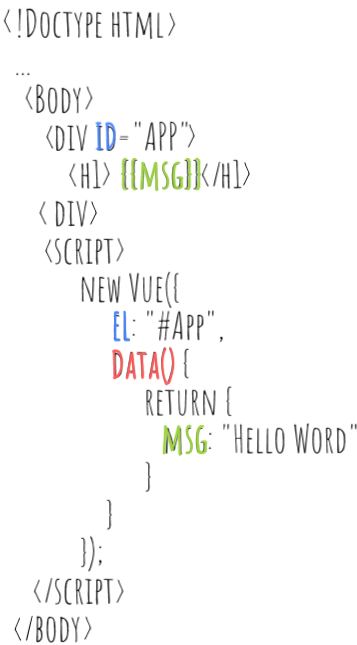
\includegraphics[scale=0.5]{fig/gettingStartedVue.PNG} 
\caption{Codebeispiel Initialisierung Vue}
\label{fig:CodeVueInit}
\end{figure} 
Zuerst muss ein Standard \ac{HTML} Dokument erstellt werden. Es enth\"alt ein \texttt{<head>} und ein \texttt{<body>} Tag. Innerhalb des \texttt{body} Tags wird ein \texttt{div} mit einer Identifikation erstellt, beispielsweise wie in Abbildung \ref{fig:CodeVueInit} mit \texttt{id=\grqq app\grqq{}}. Die Anwendung wird dort integriert. Um Daten wie einen String anzuzeigen, wird ein beliebiger Tag erstellt (zum Beispiel \texttt{h1}), der innerhalb einen Identifier besitzt, der in einer geschweiften Klammer (\texttt{<h1> \{\{msg\}\} </h1>}) steht. Um die \texttt{msg} mit einem String zu bef\"ullen, wird ebenfalls innerhalb des \texttt{body} Tags ein \texttt{<script>} Tag definiert. Hier wird eine Instanz der Vue erstellt. Die Instanz besitzt das Attribut \texttt{el}, das f\"ur die Identifikation zust\"andig ist, hei\ss{}t hier sollte \texttt{\#app} stehen. Des Weiteren hat die Vue Instanz eine \texttt{data()} Funktion, die Objekte, wie die \texttt{msg}, zur\"uck gibt.

\subsubsection*{Model-View-ViewModel}
Das Ausf\"uhren des Architekturmuster \ac{MVVM} in Vue.js hat eine deutliche und klare Abgrenzung der Komponenten und kann durch das einfache Beispiel in Abbildung \ref{fig:MVVMVue}  veranschaulicht werden.
\begin{figure}[h] 
\centering
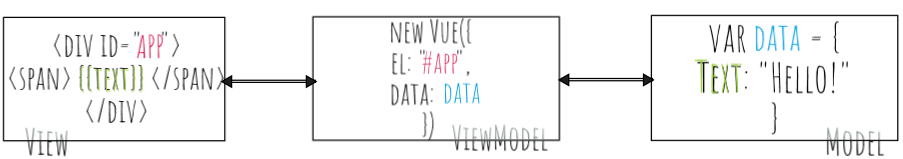
\includegraphics[scale=0.6]{fig/vueJSmvvm.PNG} 
\caption{MVVM in VueJS}
\label{fig:MVVMVue}
\end{figure} 
Die Benutzerschnittstelle, die dem Anwender dargestellt wird, wird in \ac{HTML} erfasst. In Vue.js wird dabei ein \textit{div} mit einer Identifikation, im Beispiel der Abbildung \ref{fig:MVVMVue} \texttt{app}, erstellt. In dem div soll ein Text stehen der durch das ViewModel \"ubergeben werden soll. Dieser ist, wie auch in Angular oder \"ahnlichen Templating Frameworks, mit zwei geschweiften Klammern geschrieben. 
Der Text, der an diese Stelle eingef\"ugt werden soll, wird im Model deklariert. Es wird ein Objekt erstellt, mit einem Attribut \texttt{Text}, in diesem Beispiel ein String. Das Attribut muss genauso bezeichnet werden wie das Wort innerhalb der geschweiften Klammer im \ac{HTML} Dokument.
Das Objekt wird an das ViewModel \"ubergeben und dort in die Vue Instanz \"ubertragen. In der Vue Instanz muss die Identifikation des \texttt{div} stehen und das Objekt, das an die Oberfl\"ache gegeben werden soll. Wenn das ViewModel die Instanz an das View \"ubergibt, erkennt die View die Identifikation und sucht im entsprechenden \ac{HTML} Dokument nach der passenden Identifikation. Ist das \texttt{div} gefunden, werden die Daten durchsucht und sobald dann das Attribut \texttt{Text} gefunden wurde, wird dies an der Stelle mit dem gleichen Attributsnamen eingesetzt.

 \subsection{Funktionsweise/Anwendung}
\subsection*{Routing}
In Vue.js k\"onnen Seiten durch Routing im \ac{HTML} Dokument verlinkt werden. Die Seiten werden hierzu davor definiert.
Das kann die Reaktionsf\"ahigkeit der Webanwendung deutlich verbessern, da die Seite dynamisch auf dem Kontext der Seite aufgebaut ist, bedeutet, dass die Seiten einmal geladen werden und sonst nur angezeigt werden m\"ussen und die einzelnen Bereiche aktualisiert werden, wenn sich beispielsweise Daten \"andern. Dabei m\"ussen die verschiedenen Views oder Seiten unterschieden werden. Vue.js unterst\"utzt hierf\"ur eine Router Bibliothek, \textbf{vue-router}\cite{Zynda2017}.
Um die verschiedene Seiten zu definieren und zu verlinken, wird eine Instanz des Routers erstellt, in der ein oder mehrere Routen \"ubergeben werden. Die Definition eines Routers ist ein Array, das mehrere Routen enth\"alt, mit dem Attribut \texttt{path}, das die Verlinkung zur passenden Seite enth\"alt. Diese Instanziierung wird an die Vue-Instanz \"ubergeben.
Um die Implementierung zu vollenden, muss im \ac{HTML} Dokument die Routen aufgef\"uhrt werden um sie im Web wiederzugeben. Das wird wie folgt gemacht:  \texttt{<router-view></router-view>}\cite{Bemenderfer2017}.\\

\subsection*{Templating}
Templating ist eine Vordefinierung eines Designs oder eines Formats f\"ur ein Dokument. Dies kann f\"ur Vorlagen in Word oder \"ahnliches sein, aber auch f\"ur \ac{HTML} Dokumenten als Vorlage f\"ur das Design der Webseite und Funktionen von einzelnen Komponenten. Diese Vordefinierung ist universell und kann mit jeden beliebigen Daten gef\"ullt werden\cite{DictionaryTemplating}. Templating erlaubt, Werte bzw. Daten vom Model in die View zu binden. Seit Version 2.0 wird auch JavaScript Templating mit \ac{HTML} Templating in Vue.js unterst\"utzt. \\
Das meist benutzte Symbol ist die doppelte geschweifte Klammer. Durch diese Art von Templating wird eine One-Way-Bindung vom Model zum Template aufgebaut. Mit einer One-Way-Verbindung k\"onnen Daten von dem Model zum Template gesendet werden, aber nicht von dem Template zum Model\cite{AlligatorTemplating2016}.
%TODO Abbildung
Reaktive Datenbindung ist eine der Haupteigenschaften von Vue.js, sie speichert die Daten, wie Arrays oder JavaScript Variablen, in Verbindung mit dem \ac{HTML} Dokument. Die One-Way Bindung, wie die Abbildung \ref{fig:MVVMVue} zeigt, aktualisiert das \ac{HTML} Dokument automatisch, wenn in JavaScript die \texttt{msg} manipuliert wird.\\
 Um eine Two-Way Bindung zu erzeugen und \"uber zum Beispiel einem Input Feld die Daten zu \"andern, muss an das \texttt{input} Tag ein \textbf{v-model} integriert und an die Identifikation das zu \"andernden Wertes gebunden werden. In Abbildung \ref{fig:CodeVueInit} m\"usste unterhalb der Zeile \texttt{<h1> \{\{msg\}\} </h1>} ein Input Feld mit der Bindung angef\"ugt werden (\texttt{<input v-model=\grqq msg\grqq>})\cite{Gore2016}. Wird ein neuer Text in das Input Feld geschrieben, um somit den Wert zu \"andern, wird der Wert durch die reaktive Datenbindung automatisch und mit einer geringen Reaktionszeit aktualisiert.

\subsection*{Events}
Die Autoren Etzion und Niblett erkl\"aren in ihrem Buch \enquote{Event processing in action} ein Event folgenderma\ss{}en:
\begin{quotation}
\enquote{ An event is an occurrence within a particular system or domain; it is
something that has happened, or is contemplated as having happened in that
domain. The word event is also used to mean a programming entity that represents such an occurrence in a computing system\cite{Etzion&Niblett2011}.}
\end{quotation}
Das bedeutet, dass ein Event auftritt, wenn etwas passiert, wie beispielsweise ein Mausklick bzw. das dr\"ucken auf einen Bildschirms oder das Scrollen.
Um ein Event in unser \ac{HTML} Dokument an  wie in etwa ein Button zum Klicken zu binden, wird in Vue.js ein \texttt{v-on} verwendet. Hierbei k\"onnen auf verschiedene Art und Weise ein Button oder Methoden, die ausgef\"uhrt werden sollen, gebunden werden.\\
F\"ur einen Button ist die \texttt{click}-Methode die standardgem\"a\ss{}e Weise des Events. F\"ur das folgende Beispiel wird ein Button zum hochz\"ahlen einer Zahl verwendet: \texttt{<button v-on:click=\grqq counter += 1\grqq>{{counter}}</button>}\cite{VueDokumentationEvent2018}. Das Klick-Event wird an den Button gebunden, sodass die Variable \texttt{counter} beim Eintreten des Events ver"andert wird.\\
Statt das Event an ein Objekt zu h\"angen, kann \texttt{v-on} auch an Methoden gebunden werden, um eventuell komplexere Ausf\"uhrungen durchzuf\"uhren. Dabei  kann ebenfalls eine \texttt{click}-Methode verwendet werden, die auf den Namen der Methode, die ausgef\"uhrt werden soll, hinweist (\texttt{v-on: click=\grqq Methodennamen\grqq})\cite{VueDokumentationEvent2018}. Zus\"atzlich k\"onnen Parameter in dem Methodennamen angegeben werden, die in der Methode interpretiert werden k\"onnen. 
Ebenso werden sogenannte \textit{Modifier} von Vue.js unterst\"utzt, um die immer wiederkehrenden Aufrufe w\"ahrend den Events handzuhaben.
Modifiers sind Schl\"usselw\"orter, die den Grad des Zugriffsrechts und die Sichtbarkeit auf Variablen, Funktionen oder Klassen regeln.
Ein Beispiel w\"are das \texttt{preventDefault}, das typischerweise aufgerufen wird, wenn das standardgem\"ase Verhalten des Browsers verhindert werden soll \cite{VueDokumentationEvent2018}.

\subsection*{Validation}
Eine Validierung durchzuf\"uhren, ist vor allem bei Formularen und Registrierungen wichtig. Die Validierung \"uberpr\"uft die Richtigkeit der Daten und die Erf\"ullung der gegebenen Anforderungen. Browser besitzten \"ublicherweise nativ die Validierung einer Form, da jedoch jeder Browser Objekte unterschiedlich handhaben k\"onnen, ist die Vue.js basierte Validierung eine gute L\"osung, um einheitlich zu bleiben. Zu Beginn sollte in dem \ac{HTML} Dokument ein \texttt{form} Tag vorhanden sein, ?indem die Felder zur interaktiven Anwendung eines Formulars hinzugef\"ugt werden?. Durch das schon bekannte \texttt{v-model} k\"onnen Bedingungen an ein Attribut gebunden werden und in JavaScript anhand dessen verarbeitet werden k\"onnen.
Standardgem\"a\ss{} kann bei Eingabe einer Zahl, das \"uber das \texttt{type} Attribut \"uberpr\"uft werden kann, ein Minimum und Maximum angegeben, das dann in Vue.js mit einem \texttt{v-if} \"uberpr\"uft wird und die passende Nachricht an den Anwender weiter gegeben werden kann. Diese Validierung erfolgt haupts\"achlich in JavaScript, Clientseitig oder Serverseitig. Dabei gibt es Plugins, wie Vee-Validate und Vuelidate, die schon bestimmte Regeln mit sich bringen und das Validieren in Vue.js vereinfachen\cite{VueDokumentationValidierung2018}.\\
Mit Vee-Validate wird Clientseitig validiert und durch das Hinzuf\"ugen von einem \texttt{v-validate} Attribute, das auf das Model, das \"uberpr\"uft werden soll, weist. Vee-Validate bringt eigene Regeln mit, die mit \texttt{data-vv-rules} auf das jeweilige Model angepasst werden kann\cite{BemenderferVeeValidate2017}.\\
Vuelidate ist eine Modelbasierte Validierung, was eine flexiblere, auf das Minimum  reduzierte M\"oglichkeit der Validierung ist. In dem von Vuelidate eigenen \$v Schema werden die Validierungsm\"oglichkeiten gespeichert (\texttt{this.\$v[propertyName]}). Das kann in dem \ac{HTML} Dokument durch \texttt{v-if=\grqq !\$v.emailValue.required\grqq} auf Vorhandensein \"uberpr\"uft werden. Ebenso kann eine eigene Validierung erstellt werden, wenn die gew\"unschte \"Uberpr\"ufung nicht vorhanden ist, indem  sie als Funktion dargestellt wird\cite{BemenderferVuelidate2017}.

\subsection*{Komponente}
Komponenten sind im Allgemeinen gesprochen Bereiche bzw. Teile eines Systems, die zusammen arbeiten k\"onnen.
In Vue.js helfen Komponenten, das standard-\ac{HTML} Dokument zu erweitern. 
Um ein Komponent zu erstellen, muss dies erstmals mit \texttt{Vue.component(tag, constructor)} registriert werden, um die Komponente nutzen zu k\"onnen\cite{VueDokumentationComponents2018}. In dem Konstruktor wird die Funktion definiert, die beim Verwenden des Komponenten ausgef\"uhrt wird, bzw. die Optionen mit den beinhaltenden Daten f\"ur das \ac{HTML} Dokument. Eine Option, die vorhanden sein muss, ist die option \texttt{data}. \texttt{data} sollte f\"ur die Wiederverwendbarkeit eine Funktion sein, die das unabh\"angige Objekt zur\"uck geben kann. Ist data keine Funktion, wird f\"ur jedes seperat erstellte Komponent das gleiche ausgef\"uhrt. Die Wiederverwendung kann per Name, der als \texttt{tag} \"ubergeben wird, definiert werden. Hei\ss{}t, wenn eine eigene Button-Komponente erstellt wird, kann man sie mehrmals verwenden, \textsc{Beispiel} die jedoch jeweils f\"ur sich ein eigener Button ist und die Funktion, die hinter der Komponente steht, wird f\"ur jeden Button seperat ausgef\"uhrt, da die Instanz jedes mal aufs neue erstellt wird\cite{VueDokumentationComponents2018}.
\subsection{Reactive Programming}
Reactive Programmierung wurde in den letzten Jahren immer mehr zum Trend\cite{Bainomugisha2013}. Reactive Programmierung ist ein Programmierstil, der vor allem in event gesteuerten und interaktive Anwendungen gut genutzt wird. Bekannte Unternehmen wie Amazon\footnote{https://www.amazon.de/p/feature/j5d6uh4r8uhg8ep} und Netflix\footnote{https://help.netflix.com/de/node/68708} benutzen bereits reaktive Programmierung. Dabei werden Zustands\"anderungen f\"ur das System bekannt gemacht. Wenn zum Beispiel eine Funktion aufgerufen wird, die zwei Zahlen addiert, w\"urde in dem \"ublichem Programmierstil (\textit{imperativ}) die Funktion die Variable der Summe \"andern. Wenn nach der Ausf\"uhrung der Funktion die Variablen sich \"andern w\"urden, h\"atte das keinerlei Auswirkungen auf die Summenvariable. Bei einem reaktiven Programmierstil nimmt die Summenvariable den aktuellen Wert der beiden addierten Variablen an\cite{Lambert2016}. \\
Reactive Programming ist ein Teil aus Objektorientierter und ein Teil aus Funktikonaler Programmierung, das asynchrone und immutable Streams von Events beinhaltet. Die Streams werden miteinander kombiniert und werden von \texttt{Observables} \enquote{abgeh\"ort}. 
%TODO besser erklären
%Bei einer \"ublichen Iteration k\"onnen jederzeit die Elemente, beispielsweise einer Liste ausgelesen werden, dabei wird der Zustand(engl \enquote{state}) des Objektes preisgegeben (\textit{pull}). ???Im n\"achsten Schritt werden die \texttt{Observables} an die Daten registriert und kann die Ver\"anderung der Daten an den \texttt{Subscriber} \textit{pushen}, somit kann das Programm ohne Zustand eines Objektes auskommen und die Ver\"anderung aktualisieren\cite{Lohmuller2016}???. Dies geschieht \"uber die Operationen \texttt{map, filter} und \texttt{skip}\cite{Lee2016}.
%Wenn somit ein \texttt{Pull} ausgef\"uhrt wird, darf der Nutzer entscheiden, wann er die Daten vom Erzeuger(engl. \textit{Producer}) bekommt. Das ist in die \"ublichen JavaScript Funktionen integriert. Beim \texttt{Push}, das die  \texttt{Obersvables} nutzen, ist dies genau anders herum. Der Nutzer wei\ss{} in diesem Fall nicht, wann er die Daten bekommt. In JavaScript w\"aren es \texttt{Promises}, welche die  \texttt{Push} Funktion nutzen. Ein  \texttt{Promise} gibt den Wert zur\"uck, sobald er die Daten empfangen hat\cite{Gruijs2017}.\\
Jedoch muss bei den \texttt{Observable} zwischen \texttt{Hot} und  \texttt{Cold Observables} unterschieden werden.
Cold \texttt{Observables} sind mit Listen vergleichbar, da wie gewohnt bei der Erzeugung die Gr\"o\ss{}e fest steht und der Inhalt dementsprechend nicht ver\"andert werden kann.
Hot \texttt{Observables} sind das genaue Gegenteil, hierbei ist nicht bekannt, wie der Inhalt aussehen k\"onnte oder wie gro\ss{} das Objekt wird. Hierbei wird ein Zeitintervall erstellt, dass innerhalb der angegebenen Zeit ein Event sendet, an das sich das Objekt abbonieren (engl. \textit{subscriben}) und somit Ver\"anderungen der Daten registrieren kann.\cite{Lohmuller2016}. Diese ganze Verarbeitung l\"auft in der reaktiven Programmierung asynchon ab und macht die Programme effizienter. Bei einer asynchronen Verarbeitung wird im Gegensatz zur synchronen Verarbeitung nicht gewartet , bis das Ergebnis einer Methode zur\"uck gegeben wird, sondern l\"auft im Code weiter. Das Ergebnis wird sobald es vorhanden ist zur\"uck gegeben.

\subsection*{Reaktives System}
Um die Anforderungen, Ziele und den Aufbau eines Reaktives System zu definieren, wird ein Manifest geschrieben. F\"ur das Reactive Programming hei\ss{}t das Manifest \enquote{\textit{Reactive Manifesto}}\cite{ReaktiveManifest2014}.
Oftmals werden reaktive Systeme als schneller und robuster bezeichnet, dass sich mit den vier Eigenschaften beschreiben l\"asst:
\begin{itemize}
\item \textbf{Responsive:} Die Antwortbereitschaft des Systems und die Erkennung von Bugs ist unmittelbar\cite{Lohmuller2016}. Die Fehler k\"onnen jedoch nur durch Abwesenheit einer Antwort garantiert erkannt werden, au\ss{}erdem sollten hierf\"ur die Zeit bis zur erwarteten Antwort eingegeben werden\cite{ReaktiveManifest2014}.

\item \textbf{Resilient:} Die Widerstandsf\"ahigkeit des Systems wird bewiesen durch die immer noch vorhandene Antwortbereitschaft w\"ahrend eines Systemfehlers oder von Ausf\"allen von Hard- oder Software. Implementiert werden kann dies durch Isolation von Komponenten, Eind\"ammung von Fehlern, Replikation von Funktionalit\"atem und das Delegieren der Verantwortungen\cite{ReaktiveManifest2014}. Anfragen warten in einer bestimmten Zeit auf eine Antwort, wenn diese nicht kommt, wei\ss{} der Service, der die Anfrage gestellt hat, bescheid und kann ihn zeitnah behandeln\cite{Lohmuller2016}.

\item \textbf{Elastic:} Elastisch bedeutet, dass das System auch durch verschiedene Lastbedingungen einen konstanten Service liefert. F\"ur die Erkennung der Ver\"anderungen und das darauf reagiert werden kann, muss auch hier die Replikation von Funktionalit\"aten gegeben sein. Bei erh\"ohter Last werden die Replizierungsfaktoren darauf angepasst, dabei sollten keine Einschr\"ankungen vorhanden sein\cite{ReaktiveManifest2014}. Cloud-Dienste sind hier eine gute L\"osung, um die Problematik einzugrenzen und das System kosteneffektiv zu betrieben\cite{Lohmuller2016}.

\item \textbf{Message Driven:} Nachrichtenorientierte Systeme benutzen eine asynchrone Nachrichtenkommunikation. Dabei werden die Komponente, die miteinander kommunizieren, entkoppelt und Isoliert. Dabei k\"onnen Fehler an andere eventuell \"ubergeordnete Komponente gesendet werden. Die Systeme lassen sich an die Nachrichten h\"angen, was die \"Uberwachung von Ver\"anderungen verinfacht\cite{Lohmuller2016}. Die Nachrichten\"uberwachung veranlassen einen \"Uberblick \"uber das Laufzeitverhalten des Systems und der \"ubermittelten Nachrichtenfl\"usse. Bei Nachrichtenorientierte Systeme ist das Programm auch ortsunabh\"angig m\"oglich, bedeutet, dass Teile des Codes nicht auf demselben Computer ausgef\"uhrt werden m\"ussen\cite{ReaktiveManifest2014}.
\end{itemize}

\begin{figure}[h] 
\centering
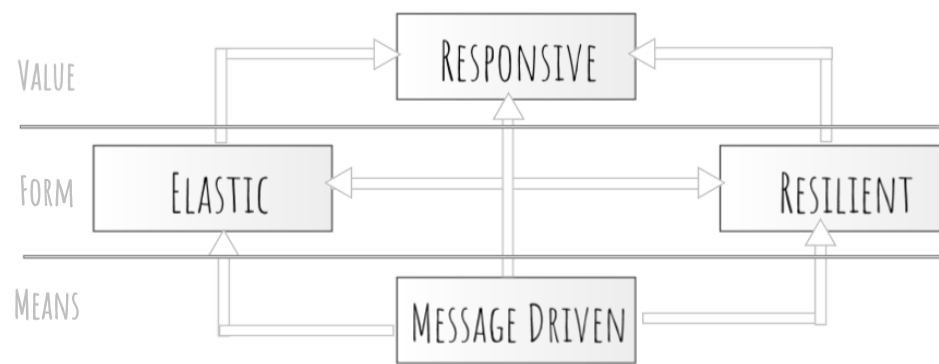
\includegraphics[scale=0.5]{fig/reaktiveSystem.png} 
\caption{Zusammenspiel reaktives System}
\label{fig:RS}
\end{figure} 

Auf Abbildung \ref{fig:RS} wird das Zusammenspiel der vier reaktiven Qualit\"aten illustriert.
In gro\ss{}eren Anwendungen gibt es mehrere Komponenten, die voneinander abh\"angig sind. Deshalb m\"ussen die vier Qualit\"aten in jeder Ebene des Gesamtsystems ber\"ucksichtigt werden und es somit innerhalb der Schichten kombinierbar\cite{ReaktiveManifest2014}.
Zur Umsetzung eines reaktiven Programms gibt es Frameworks, die die Anforderungen, Eigenschaften und Ziele eines reaktiven Programmes helfen umzusetzen. Beispiele hierf\"ur w\"aren Vue.js, React.js und weitere.
\subsection{Andere Frameworks}
Analog zu Vue.js gibt es weitere Bibliotheken bzw. Frameworks, die die Anforderungen ebenfalls als Reactive Programming betreiben und mit dem Entwurfsmuster \ac{MVVM} arbeiten. Ein Beispiel w\"are \textbf{React.js}.
React.js ist ein von Facebook erstellte JavaScript Bibliothek, das dem Entwickler beim Erstellen von Oberfl\"achen hilft. Konzerne wie Whatsapp, Instagram und Facebook nutzen die Frontend Bibliothek. Das Ziel, das React.js verfolgt, ist es einfacheren Code zu schreiben, um die einzelnen Bestandteile besser zu verstehen und weniger komplex zu halten. Die wesentliche Bestandteile von React.js sind die Komponentenarchitektur, der virtuelle \ac{DOM} und die Browserkompatibilit\"at.\\
React.js Komponente sind \"aquivalent zu Web Komponenten, die mit \texttt{React.createClass} erstellt werden. Innerhalb gibt es Funktionen wie \texttt{render}, die das \ac{HTML} Dokument f\"ur das Web pr\"asentierbar machen. Dazu k\"onnen eigene Funktionen definiert werden. Bei React.js wird die standard \texttt{onClick} Methode als Attribut auf den Button gesetzt und durch geschweifte Klammer kann auf die Funktionen verwiesen werden (\texttt{<button onClick={this.add}>}). Ein besonderes Attribut von React.js ist das \texttt{State}. Dieses Attribut beinhaltet die zu ver\"andernden Daten und kann die Aktualisierung im \ac{HTML} Dokument durchf\"uren. Somit muss auf die Anpassung des \ac{DOM} keine R\"ucksicht genommen werden. Die Komponente werden in React.js innerhalb der \texttt{render} Methode definiert, da React.js JSX eine schlanke Syntaxerweiterung zum Schreiben von Markups verwendet. \"Anderungen am Stil der Seite oder des Buttons wird innerhalb der \texttt{createClass}, wo auch die \texttt{render} Methode f\"ur die Definition des \ac{HTML} Dokuments implementiert wird, erstellt (\texttt{return {backgroundColor: \#fff};}). Hierbei wird erkannt, dass die \"ublich bekannte Trennung der Bereiche \ac{HTML}, \ac{CSS} und JavaScript nicht stattfindet\cite{Kogel2015}. \\
Die Bearbeitung durch JSX in React.js wird in der Regel nicht direkt in dem \ac{DOM} des Browsers stattfinden, sondern mit einem virtuellen \ac{DOM}, das ein JavaScript Objekt ist, das zur Bearbeitung genutzt wird. Bei einer Ver\"anderung wird jeweils ein neues Objekt, also ein neuer virtueller \ac{DOM}, erstellt. Dabei wird der virtuelle \ac{DOM} mit dem Browser \ac{DOM} verglichen und aufgelistet. Die \"Anderungen werden erst zum Zeitpunkt des Batch an den Browser geschickt und aktualisiert\cite{Skirzynski2015}. Im Vergleich zu Vue.js ist React.js einer der \"ahnlichsten Bibltiotheken. Beiden nutzen einen virtuellen \ac{DOM}, eine reaktive, zusammensetzbare Benutzeroberfl\"ache und nutzen durch das Routing und des States um die \"Anderungen zu fokusieren. Die folgende Auflistung zeigt die Unterschiede in Vue.js und React.js in den Positionen der Leistung, im Templateing und JSX und die Skalierbarkeit des Systems.
\begin{itemize}
\item \textbf{Leistung:} Vue.js und React.js sind in Hinsicher der Leistung \"ahnlich schnell, was f\"ur die Entscheidung irrelevant ist. Die genauere Leistung wird im sp\"ateren Teil genauer bezeichnet\cite{VueDokumentationOther2018}.
\item \textbf{Templating} Im Gegensatz zu Vue.js ist in React.js \ac{HTML} und \ac{CSS} zusammen in JavaScript mit Hilfe von JSX geschrieben, das mit Hilfe einer \texttt{render} Funktion, die ebenfalls in Vue.js vorhanden ist, an der Benutzeroberfl\"ache daregestellt werden kann. Ebenso werden Werkzeuge wie Typen\"uberpr\"ufung in React.js besser unterst\"utzt\cite{VueDokumentationOther2018}. Die konkrete Teilung zwischen JavaScript, \ac{HTML} und \ac{CSS} ist in Vue.js deutlich erkennbar und f\"ur die Meisten Entwickler \"ubersichtlicher\cite{Haupt2018}. In Vue.js ist das Templating f\"ur das Rendering des \ac{HTML} Dokuments. F\"ur viele Entwickler, die in \ac{HTML} Erfahrung haben, wird es einfacher sein, den Code zu lesen und zu interpretieren\cite{VueDokumentationOther2018}.
\item \textbf{Skalierbarkeit:} F\"ur die Skalierung f\"ur gr\"o\ss{}ere Anwendungen gibt es in Vue.js sowie in React.js viele Routing L\"osungen. In React.js gibt es die Frameworks Fluex oder Redux und in Vue.js das Vuex, auch Redux kann in Vue.js integriert werden\cite{Peters2017}. Vue.js beinhaltet einen \ac{CLI}, das die Einbindung neuer Projekte mit Werkzeugen zum Bauen des Projekts wie webpack oder Browserify erm\"oglicht.
Vor allem in React.js m\"ussen die Build Systeme, zum Bauen des Projekts sich zuerst angeeignet werden, was in Vue.js beispielsweise das Webpack \"ubernimmt\cite{VueDokumentationOther2018}.
\end{itemize}
Ein weiteres Framework, das f\"ur die Frontend Entwicklung hilfreich ist, ist \textbf{Angular.js}. Angular.js ist den Meisten bekannter als Vue.js oder React.js. Viele Komponenten oder Syntaxen von Angular.js waren f\"ur Vue.js Inspirationen, weshalb es vielen Angular.js Entwicklern einfacher f\"allt sich in Vue.js einzuarbeiten. Angular.js ist deutlich komplexer und hat mehr Vorgabe in Hinsicht der Softwarearchitektur als Vue.js. Ebenso ist die Leistung von Vue.js deutlich besser und leichter zu optimieren. 
Die Entscheidung f\"ur Vue.js basierte auf der immer gr\"o\ss{}erer werdenden Popularit\"at seit 2016, was durch die Google Trends Statistik deutlich hervorgeht\cite{GoogleTrends2018}.  F\"ur die Gr\"o\ss{}e des zu implementierende Projekt ist Angular.js zu \"uberladen. Vue.js oder React ist kompakt genug, f\"u eine Webanwendung zur Darstellung von Positionsdaten jedoch ausreichend. Dabei ist die Leistung sehr entscheidend. \newline
in einer Studie einer Bachelorarbeit aus Schweden wurde der Performancevergleich von Angular 2, Aurelia,  Ember, Vue und weiteren getestet. Dabei wurden die Befehle \texttt{Create}, \texttt{Delete} und \texttt{Update} mit jeweils 1000 Reihen getestet.\cite{Svensson2015}
\begin{itemize}
\item \textbf{Angular.js 2:} Im Ganzen hatte Angular 2 in jedem Testszenario die beste Leistung, dabei hat Angular 2 eine deutliche Verbesserung zu seinem Vorg\"anger 1.5\cite{Svensson2015}.
\item \textbf{Aurelia:} Aurelia hat in dem Szenario das zweitbeste Ergebnis erziehlt, jedoch schnitt Aurelia bei dem Befehl Update mit unter Anderem als schlechtestestes Frameworks ab\cite{Svensson2015}.
\item \textbf{Ember:} Eins der schlechtesten Frameworks ist Ember. Nur in dem Befehl Delete erreichte Ember einen durchschnittliches Ergebnis\cite{Svensson2015}.
\item \textbf{Vue.js:} Vue.js war eins der schnellsten Frameworks, vor allem bei den Befehlen Create und Update\cite{Svensson2015}.
\end{itemize}


\section{Architekturmuster Model-View-ViewModel}
\subsection{Motivation}
Naveen Pete, ein Online-Blogger, bezeichnete ein Architekturmuster, auch Entwurfsmuster genannt, als ein \enquote{gut strukturiertes Dokument}, dass als L\"osung f\"ur wiederkehrende Probleme dienen soll\cite{Pete2016}.
\begin{quotation}
\enquote{A design pattern is a well-documented solution to a recurring problem.}
\end{quotation}
Architekturmuster werden zur sauberen Trennung der Anwendungslogik und der Benutzeroberfl\"ache genutzt. Das vereinfacht das Testen, die Instandhaltung und das Weiterentwickeln der Software. Au\ss{}erdem verbessern Architekturmuster die Wiedernutzung des Codes f\"ur Andere Projekte, da lediglich der View Part plattformspezifisch angepasst werden muss\cite{MicrosoftMVVM2012}.
Architekturmuster werden vor allem in gro\ss{}en Projekten genutzt, um eine Abgrenzung zwischen \enquote{Ansicht} und \enquote{Modell} zu schaffen. In dem Architekturmuster \ac{MVVM} ist eine klare Abgrenzung zwischen der grafischen Oberfl\"ache (View) und der Daten (Model) durch eine Schnittstelle (ViewModel) gegeben.



\subsection*{Model}
In  den \"ublichen Architekturmustern wird das Model als \enquote{Abbildung der Datenquelle} gesehen. F\"ur das  Architekturmodell \ac{MVVM} ist das Model eine Abbildung der Daten f\"ur die Visualisierung. Diese Daten werden vom Benutzer manipuliert und zur Verf\"ugung gestellt.
Das Model stellt dabei folgende Funktionalit\"aten bereit:
\begin{itemize}
\item Validierung
\item Benachrichtigungen bei \"Anderungen
\item Verarbeiten nach vorgegebenen Regeln
\end{itemize}
Was dabei zum Einsatz kommt, h\"angt von den Anforderungen an das Model ab. Werden die Daten beispielsweise von einem OR-Mapper oder einem Service zur\"uck geschickt, k\"onnten diese Funktionalit\"aten ebenso in das ViewModel implementiert werden\cite{EderModel2017}.

\subsection*{View}
Die View ist die strukturierte Benutzeroberfl\"ache, in der Daten, Videos sowie Bilder dargestellt werden und keinerlei Logik enthalten ist. Benutzereingaben, wie \"uber die Tastatur werden in der View abgefangen und an das ViewModel weiter gegeben. Die View ist ausschlie\ss{}lich mit dem ViewModel verbunden und das nur, wenn die Daten an die View \"uberreicht werden. Im Code sollte in der View so wenig wie m\"oglich geschrieben und unabh\"angig sein. Das hei\ss{}t, der Code sollte sich ausschlie\ss{}lich auf die View beziehen. Dies erm\"oglicht das einfache Austauschen der View, ohne gro\ss{}e \"Anderungen am Code zu leisten\cite{EderView2017}.

\subsection*{ViewModel}
Einfach gesagt, stellt das ViewModel das Model f\"ur die View dar und gibt das Model nach au\ss{}en, hei\ss{}t das ViewModel bearbeitet die Logik der View. 
Das ViewModel kommuniziert mit dem Model  durch Methodenaufrufe und stellt die Daten, das das ViewModel vom Model geliefert bekommt, der View dar. Die zur Verf\"ugung stehenden Funktionalit\"aten werden durch die View gebunden, wodurch f\"ur die View keinerlei Code anf\"allt.
Referenzen auf Elemente der View d\"urfen nicht erstellt und darauf zugegriffen werden, da, wie in dem Abschnitt der View bereits erw\"ahnt wurde, keine Abh\"angigkeiten erstellt werden d\"urfen. Durch Funktionen \"uber die View zu testen ist unpraktisch und entf\"allt hier, da das ViewModel selbst die Abstraktion der View die M\"oglichkeit besitzt, das abzudecken.
Das ViewModel bezieht sich niemals auf die View und kann somit auf jede View bezogen werden und macht sich daf\"ur wiederverwendbar\cite{EderViewModel2017}.
%BILD
\subsection{Model-View-ViewModel}
%TODO
Durch die Entwicklung des Windows Presentation Foundation Framework (WPF) durch Microsoft\footnote{https://www.microsoft.com/de-de} entstand 2005 das Architekturmodell \ac{MVVM}. Es ist ein fester Bestandteil von Silverlight\footnote{Silverlight is a cross-browser, cross-platform plug-in for delivering media and rich interactive applications for the Web}. Ebenso werden existierende Frameworks um \ac{MVVM} erweitert\cite{Jaeckle2015}.

\begin{figure}[H] 
\centering
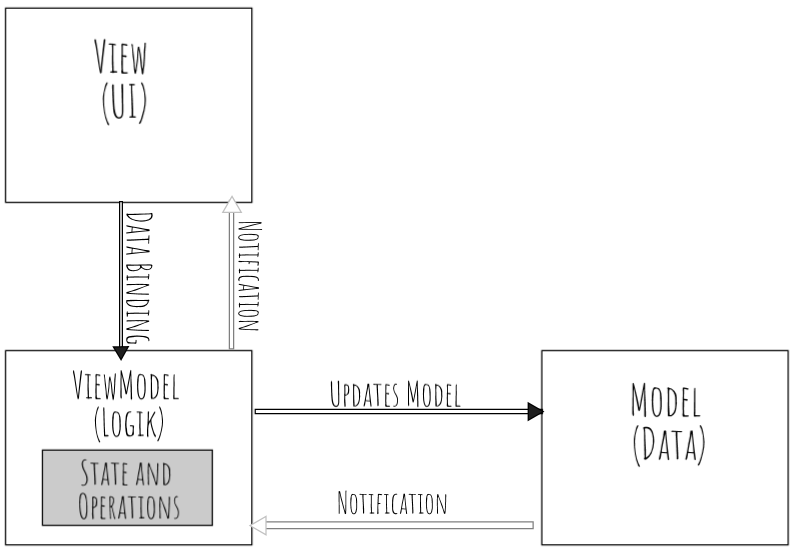
\includegraphics[scale=0.45]{fig/mvvmv2.png} 
\caption{Komponente des MVVM Architekturmusters\footnotemark}
\label{fig:MVVM}
\end{figure} 
\footnotetext{in Anlehnung an: \cite{MicrosoftMVVM2012}}
Wie die drei Komponente View, ViewModel und Models miteinander zusammenh\"angen und kommunizieren, wird im folgenden erl\"autert und durch Abbildung \ref{fig:MVVM} abgebildet.

\subsection*{Data-Binding}
Wie vorher schon erw\"ahnt wurde, kennt die View das ViewModel und das ViewModel kennt das Model, jedoch nicht vice versa, was die Pfeile in Abbildung \ref{fig:MVVM} illustriert.
Damit die View mit dem ViewModel interagieren kann, wird in WPF ein sogenanntes Data-Binding verwendet.
Durch die Datenbindung wird eine Verbindung zwischen der View (\ac{UI}, die Benutzerschnittstelle) und dem ViewModel (Logik) hergestellt. Wenn das Model (Daten) die korrekten Benachrichtigung bereitstellt, k\"onnen die eingebundenen Daten automatisch die \"Anderung des Wertes annehmen und in der View wiedergeben werden\cite{Cai2017}.
Eine Verbindung besteht zumeist aus vier Komponenten: einem Zielobjekt, einer Zieleigenschaft, die eine Abh\"angigkeitseigenschaft sein muss, einer Quelle und einem Pfad zum Wert, der verwendet wird. 
Wenn eine Verbindung aufgebaut wird, ist die Richtung des Datenflusses entscheidend. Es gibt drei verschiedene Wege die Daten zu senden bzw. zu empfangen.
\begin{itemize}
\item One-Way Bindung
\item Two-Way Bindung
\item One-Way To Source Bindung
\end{itemize}
\stepcounter{footnote} 
\begin{figure}[h] 
\centering
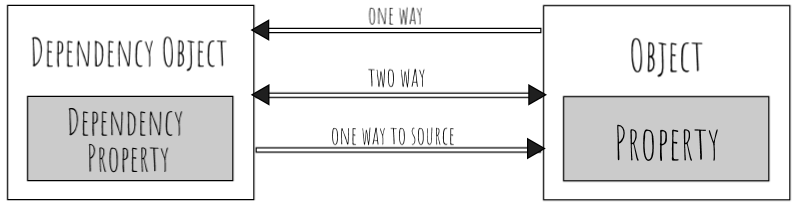
\includegraphics[scale=0.55]{fig/Data-Binding.png} 
\caption{Datenbindung zwischen View und ViewModel\footnotemark}
\label{fig:DataBinding}
\end{figure} 
\todo{Fu\ss{}noten}\\
%\footnotetext{in Anlehnung an: \cite{Cai2017}
Die View, besitzt ein Dependency(engl. f\"ur abh\"angig) Objekt mit einer Dependency Property, einer Eigenschaft, wie zum Beispiel einem String. Diese sind abh\"angig voneinander. Das ViewModel, enth\"alt ein Objekt mit einer Property. Eine One Way Bindung l\"asst \"Anderungen an der Quelle zu und aktualisiert die Zieleigenschaften automatisch. Diese Verbindung ist dann n\"utzlich, wenn schreibgesch\"utzte Elemente in der \ac{UI} vorhanden sind, denn \"Anderungen an den Zieleigenschaften sind bei einer One Way Bindung nicht m\"oglich.
Eine Two Way Bindung erm\"oglicht dem User, \"Anderungen vorzunehmen. Hierbei werden die Zieleigenschaften ver\"andert und automatisch die Quelleigenschaften aktualisiert. Andersherum geschieht dasselbe, analog zur One Way Bindung. Die kontr\"are Bindung zur One Way Bindung ist die One Way To Source Bidnung, diese aktualisiert automatisch die Quelleigenschaften wenn die Zieleigenschaft ge\"andert wurde.
\subsection*{Notifications}
Um die \"Anderung zu erkennen, muss die Quelle einen Benachrichtgungsmechanismus beinhalten. In der Regel ist dies die \texttt{INotifyPropertyChanged} Implementierung. Bei dieser Implementierung wird ein Objekt an die \ac{UI} gebunden. Hier ist das Ereignis \texttt{PropertyChanged} enthalten, dies wird ausl\"ost, sobald eine \"Anderungen an der Eigenschaft des Objektes stattfindet. Diese \"Anderung wird von dem Model an das ViewModel gesendet, das dann die Aktualisierung an der Quelleigenschaft vornehmen kann und die \"Anderung in der View angezeigt.
Die Quellaktualisierungen werden anhand \texttt{UpdateSourceTrigger}, die Eigenschaften enthalten, die bestimmen, wann und warum die Benachrichtigung ausgel\"ost wird,  ausgel\"ost. 


\subsection*{Fazit}
Das Ziel des Architekturmuster ist, wie auch bei dem Architekturmuster \ac{MVC}, dem Vorreiter von \ac{MVVM}, das Trennen der Logik und der Pr\"asentationsschicht bzw. der View.
Die Vorteile des Entwurfsmuster \ac{MVVM} sind:
\begin{itemize}
\item Durch die Trennung m\"ussen \"Anderungen, die an dem Model vorgenommen werden, nicht an der View ge\"andert werden\cite{tutorialspointMVVM} .
\item W\"ahrend der Entwicklung k\"onnen die Entwickler und die Designer unabh\"angig voneinander an den Komponenten arbeiten\cite{Pete2016}.
\item Modultests f\"ur das ViewModel und das Model k\"onnen ohne die View erstellt werden\cite{Pete2016}.
\item Die View kann beliebig ausgetauscht und wiederbenutzt werden, da die View unabh\"angig von den anderen Komponenten ist\cite{Pete2016}.
\item Die Weiterentwicklung sowie die Instandhaltung kann durch die Trennung detaillierter vorgenommen werden, ohne dass die  \"Anderungen negative Auswirkungen auf das System haben\cite{tutorialspointMVVM}.
\end{itemize}
Die Nachteile des Architekturmuster sind nicht von Relevanz.
F\"ur viele Entwickler ist \ac{MVVM} f\"ur einfache Oberfl\"achen zu m\"achtig und ebenso bei gr\"o\ss{}ere F\"alle kann es zu Problemen bei der Konstruktion des ViewModel kommen.
Wenn die Datenbindung komplexer wird, wird das Debugging problematischer\cite{tutorialspointMVVM}.


\subsection{Verwandte Architekturmuster}
\setcounter{secnumdepth}{3}
\subsubsection{Model-View Controller}
Das Hauptmerkmal des Architekturmusters \ac{MVC} ist die Trennung der View und des Controllers. Genau das macht das MVC komfortabel f\"ur Web Anwendungen und weniger geeignet f\"ur Desktop Anwendungen\cite{Syromiatnikov2014}.

\subsubsection*{Model}
Das Model ist beim Architekturmuster \ac{MVC} der Ort, an dem die Daten und Objekte sowie der Netzwerkcode gespeichert und implementiert werden. Das hei\ss{}t, der Model Part beinhaltet die Informationen, um die View anschaulich zu machen und die Logik, die die \"Anderungen des Users verarbeitet und die View damit benachrichtigt\cite{Leff2001}.
\subsection*{View}
In der View ist ebenso wie in dem \ac{MVVM} Architekturmuster keinerlei Logik enthalten, was es wiederverwendbar f\"ur andere Projekte macht.\cite{Peres2016} Die View setzt Informationen f\"ur den Anwender ins Bild. Mit dem Controller zusammen definieren sie das User Interface (Benutzerschnittstelle)\cite{Leff2001}.
\subsection*{Controller}
Der Controller vermittelt vorwiegend \"uber \enquote{delegation pattern} zwischen der View und dem Model. Delegation Pattern ist eine Technik, bei der Objekte Verhalten nach au\ss{}en darlegen und das Verhaltens an ein anderes Objekt \"ubertragen\cite{TU-Wien2013}. Idealerwei\ss{}e kennt der Controller die View nicht und kommuniziert \"uber ein bestimmtes abstraktes Protokoll\cite{Peres2016}.
Der Controller verarbeitet die Events der View und leitet sie an das Model weiter, das dann die View \"uber die \"Anderung benachrichtigen kann und die View die \"Anderung dem Anwender darstellt. Vergleichbar mit dem ActionListener in Swing\cite{Singer2004}.
\subsection*{Model-View-Controller}
\begin{figure}[h] 
\centering
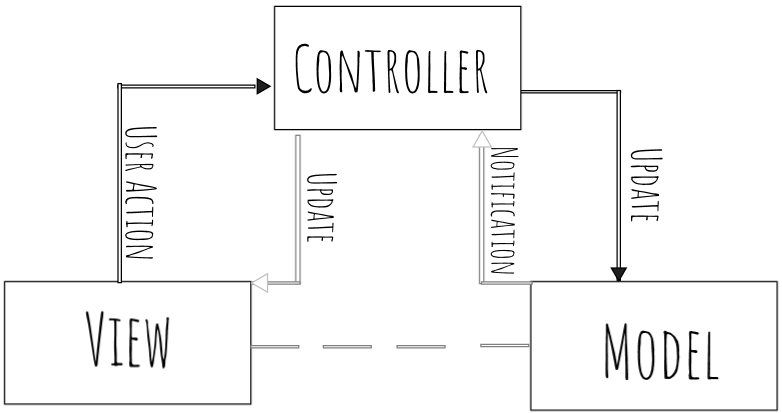
\includegraphics[scale=0.4]{fig/mvc.png} 
\caption{Komponente des MVC Architekturmusters}
\label{fig:MVC}
\end{figure} 
Auf Abbildung \ref{fig:MVC} erkennt man die Zusammenh\"ange zwischen den Komponenten des Architekturmodells \ac{MVC}. Dieses Modell l\"asst mehrere Views und Controller zu, die unabh\"angig von dem Model erstellt und modifiziert werden k\"onnen\cite{Curry2008}.
Wenn der Anwender eine Aktion in der View ausl\"ost, wird diese an den Controller geschickt, der anhand der Manipulation das Model aktualisiert. Sobald die Aktualisierung abgeschlossen ist, wird eine Benachrichtigung an den Controller gesendet, ob diese erfolgreich war oder nicht. War die Aktualisierung erfolgreich, aktualisiert der Controller anhand der Benachrichtigung die View.
\subsection*{Kommunikation}
Obwohl das Model unabh\"angig von den Views ist, sollten die Komponente miteinander kommunizieren. Ebenso die Controller und die Views. Da die View jedoch das Model kennt, kann die View mit dem Model in Kontakt treten. Die Kommunikation mit den Nachrichten findet \"uber \textbf{Events} (Aktionen) statt. Events stellen Mechanismen bereit, die mit wenigen Abh\"angigkeiten eine Kommunikation zustande kommen kann.
Grafische Komponente, wie Listen, Textfelder oder \"ahnliche k\"onnen Benachrichtigungen empfangen, beispielsweise wenn geklickt wird. Diese Benachrichtigungen kommen in der Regel vom Controller. Die View registrieren die Events an Objekte, die sie bearbeiten m\"ochten. Wenn die Nachricht zum Model gesendet wurde, wird das Application Model auf diese Nachricht antworten, die Daten aktualisieren und eine Nachricht zur\"uck senden. Das Application Model kann ebenso events ausl\"osen und somit die abh\"angigen Views \"uberwachen\cite{Deacon2005}. 
%F\"ur die Benachrichtigung vom Application Model zur View und umgekehrt ist der Controller zust\"andig, da der Controller die Anfragen des Anwenders interpretiert.


\setcounter{secnumdepth}{3}
\subsubsection{Model-View Presenter}
Das Architekturmuster \ac{MVP} basiert auf dem \ac{MVC} Muster. Die Komponente wurden anhand hohen Flexibilit\"at angepasst und die M\"angel des vorherigen Musters (\ac{MVC}) werden besser gehandhabt.  Das Hauptmerkmal des \ac{MVP} Musters ist der Presenter, der direkten Zugriff auf die View und das Model besitzt und deren Zusammenspiel handhabt. Die View und das Model k\"onnen kleine Situationen selbst meistern, was das ganze die Komplexit\"at des Presenters reduziert, da dieser nur noch f\"ur die komplexen Anforderungen verantwortlich ist. Somit ist das Architektumuster \ac{MVP} das flexibelste der MV* Familie, da es dem Entwickler viel Freiraum und Kontrolle gibt. Zum Beispiel kann die Datenbindung da genutzt werden, wo es dem Entwickler am besten passt\cite{Syromiatnikov2014}.
Die Views sind wie auch beim \ac{MVC} Muster f\"ur die Anschauung der Daten zust\"andig und das Model f\"ur die Datenhaltung verantwortlich. Martin Fowler verglich 2006 das Architekturmuster \ac{MVC} mit \ac{MVP} so, dass der Controller in \ac{MVC} bei  \ac{MVP} ein Teil der View ist\cite{Bragge2013}. Die Reaktion auf die Aktivit\"aten des Users ist im Presenter enthalten. Er kann entscheiden wie das Model manipuliert und ver\"andert werden kann, hei\ss{}t er \"ubernimmt bzw. integriert die Rolle des Application Model, das man von \ac{MVC} kennt. Zusammenfassend zu sagen ist, dass der Presenter die Business Logik zur Verf\"ugung stellt.
In der Regel verh\"alt sich die Kommunikation gleich wie beim \ac{MVC}. Durch Aktionen des Anwenders, wie eine Mausbewegung, werden \texttt{Interactor Events} ausgel\"ost. \textbf{?} Diese Interactionen werden vom Presenter interpretiert\cite{Potel1996}.




 
\subsection{Fazit}
Bevor Software-Projekte mit Architekturmuster realisiert worden waren, wurde die grafische Oberfl\"ache in die Mitte der Anwendung implementiert. Dieser einfache Einsatz wird Smart \ac{UI} anti-pattern genannt, das wie jedes Muster seine Vorteile hat, aber bei gr\"o\ss{}eren Projekten zu einer H\"urde werden kann. Das Gestalten der verschiedenen Architekturmustern bew\"altigen die Probleme des Smart \ac{UI} anti-pattern. Jedes Architketurmuster ist \"ahnlich aufgebaut, jedes trennt die Benutzerschnittstelle mit den Daten und deren Verarbeitung. Die Kommunikation zwischen den drei Komponenten h\"angt von der grundlegenden Umgebung ab. Beispeilsweise ist die Synchonisation mehrerer Views durch einen \texttt{\enquote{observer}}, einen Beobachter, der die \"Anderungen weitergibt und somit die View aktualisiert, n\"utzlich, aber in vielen Situationen nicht zug\"anglich. Somit sind auch andere Mechanismen brauchbar, wie die Datenbindung die in dem Architekturmuster \ac{MVVM} zwischen dem ViewModel und der View. Die Anwendung des Mechanismus zur Kommunikation h\"angt von der Anwendung selbst, der Programmiersprache, der Frameworks, des angewendeten Musters und der pers\"onlichen Preferenz aufgezeigt\cite{Bragge2013}. In der folgenden Tabelle\cite{Syromiatnikov2014} werden die Vorteile und Nachteile des jeweiligen Entwurfsmusters. Dies zeigt, dass kein Gewinner ausgew\"ahlt werden kann, jeder hat seine eigenen individuellen Vorz\"uge.
\begin{table}[h]
\centering
\caption{Vorteile und Nachteile der Architekturmuster}
\label{ProConsPattern}
\begin{tabular}{p{2cm}p{7cm}p{7cm}}
\toprule
Muster & Vorteile & Nachteile \\ \midrule
\ac{MVVM}              
& Unterst\"utzt mehrere Views f\"ur das gleiche Model und aktualisiert View und ViewModel automatisch
& 
Das Benutzten von \enquote{Beobachter} schw\"acht die Leistung. Beruht auf der zugrunde liegenden Technologie.  \\ \hline
\ac{MVC}     
 & 
Gut geeignet f\"ur Web Anwendungen, da View und Controller hier getrennt gehandhabt wird.
 &
 Die Abh\"angigkeit von View und Controller, was hier nicht gegeben ist, sind in manchen Steuerelementen von n\"oten.  \\ \hline
\ac{MVP}            
&
Flexibilit\"at und Freiheit zum Verwenden der verschiedenen Mechanismen und kann an viele Anwendungsszenarien verwendet werden. 
&
Keine strikte Trennung der Komponenten, das bei komplexere Codestellen zu Problemen f\"uhren kann.  
\\ \bottomrule
\end{tabular}
\end{table}
 

\section{Requirements}

\subsection{Top-Level Requirement}
\begin{itemize}
\item \textbf{Top Requirement 1000:}\\
Das System C.A.M. soll die Lage eines Fahrzeuges \"uber eine Deckenkamera auf der Fahrbahn ermitteln und zur Visualisierung bereitstellen.
\end{itemize}

\subsection{Geforderte Anwendungf\"alle}

\begin{itemize}
\item \textbf{Anwendungsfall Tracking:}\\
Das System soll das Fahrzeug auf der Fahrbahn erfassen.
\item \textbf{Anwendungsfall Darstellung:}\\
Das System soll die Fahrzeugposition auf der Fahrbahn visuell darstellen.
\end{itemize}

\textbf{Anforderungen an den Anwendungsfall "Tracking"}
\begin{itemize}
\item  \textbf{Requirement 2100:}\\
Das System muss das Fahrzeug erkennen.
\item \textbf{Requirement 2200:}\\
Das System muss die Position des Fahrzeugs erkennen.
\item \textbf{ Requirement 2300:}\\
Das System muss die Richtung des Fahrzeugs erkennen.
\item\textbf{ Requirement 2400:}\\
Das System muss die Geschwindigkeit des Fahrzeugs erkennen.
\item \textbf{Requirement 2500:}\\
Das System muss die ermittelten Daten \"uber eine Schnittstelle ausliefern.
\end{itemize}

\textbf{Anforderungen an den Anwendungsfall "Darstellung"}
\begin{itemize}
\item \textbf{Requirement 3100:}\\
Das System muss als Webanwendung implementiert werden.
\item \textbf{Requirement 3200:}\\
Das System muss die Fahrbahn visualisieren
\item \textbf{Requirement 3300:}\\
Das System muss anhand der \"ubermittelten Daten das Fahrzeug auf der Fahrbahn visualisieren
\end{itemize}

\subsection{Anforderungen an die technischen Funktion}
\textbf{Anforderungen an Start-up und Shut-down}
\begin{itemize}
\item \textbf{Requirement 1100:}\\
Nach dem Starten des Systems m\"ussen alle Funktionen zur Verf\"ugung stehen.
\end{itemize}

\textbf{Anforderungen an die Fehlererkennung, -behandlung und -ausgabe}
\begin{itemize}
\item \textbf{Requirement 1200:}\\
Alle Fehler die w\"ahrend des Betriebs des Systems entstehen, sollten protokolliert und
gespeichert werden.
\item \textbf{Requirement 1210:}\\
Geht das System in einen undefinierten, unsicheren Zustand \"uber, sollte es automatisch in einen sicheren Zustand gebracht werden.
\end{itemize}

\textbf{Anforderungen an die Kommunikation}
\begin{itemize}
\item \textbf{Requirement 1300:}\\
Es sollen die ermittelten Fahrzeuginformationen von dem Tracking zu der Darstellung mittels eines Websockets \"ubertragen werden.
\item \textbf{Requirement 1400:}\\
Die externe Deckenkamera soll die Bilder \"uber eine USB-Schnittstelle an das System\"ubertragen.
\end{itemize}

\textbf{Anforderungen an die Qualit\"aten}
\begin{itemize}
\item \textbf{Requirement 1520:}\\
Das System soll im Bereich Mehrfachdetektion von Fahrzeugen sowie von Hindernissen erweiterbar sein.
\item \textbf{Requirement 1530:}\\
Das System soll die Mehrfachdetektion von Fahrzeugen sowie von Hindernissen visuell erweiterbar sein
\item \textbf{Requirement 1540:}\\
Das System soll die Fahrzeuge steuern k\"onnen
\end{itemize}
\chapter{Teilsystem Visualisierung}
\label{sec:TeilVisu}
\section{Anforderungen an das Teilsystem}
Requirements, in deutsch \enquote{Anforderungen}, beschreiben die Ziele eines Kunden, die angeforderten Funktionalit\"aten und Eigenschaften des Systems, sowie in welcher Qualit\"at dies umgesetzt werden muss\cite{Heini2010}. Die Beschreibung, das Pr\"ufen, das Verwalten sowie die Analyse solcher Requirements wird als des Requirements Engineering beschrieben\cite{Sophist2011}. \par\smallskip 
Dieses Kapitel definiert die funktionalen und nicht-funktionalen Anforderung an das Teilsystem. Die Anforderungen wurden nach dem selben Prinzip, welches zu Beginn in Kapitel \ref{sec:req} beschrieben wurde, erstellt.

\subsection*{Funktionale Requirements}
Funktionale Requirements charakterisieren die Leistungen an das System von Anwendungsf\"allen. Zus\"atzlich definieren die funktionalen Requirements die technischen Funktionen eines Systems, die als L\"osung f\"ur die Problematik der Anwendungsf\"alle fungieren\cite{Goll2011}.
\subsection*{Funktionales Top Level Requirement}
\textbf{Requirement 1000:}\\
Das System muss Anwendern eine Fahrbahn visualisieren und die darauf vorhandene Position eines Fahrzeugs aufzeigen.
\subsection*{Requirements an die Anwendungsf\"alle}
\begin{itemize}
\item \textbf{Requirement 1110:}\\
Der Anwender soll das Fahrzeug vom System aus ein- und ausschalten k\"onnen.
\item \textbf{Requirement 1120:}\\
Der Anwender soll durch Eingabe einer Zahl die Geschwindigkeit des Fahrzeugs anpassen.\\
\end{itemize}

\subsection*{Nicht funktionale Requirements}
Nicht funktionale Requirements definieren Forderungen an den L\"osungsbereich wie die Architektur, Technologien oder an die Qualit\"at wie zum Beispiel die Performance. Beispiele hierf\"ur sind sie Bedienbarkeit, das eingesetzte Betriebssystem, die verwendete Hardware und die genutzte Programmiersprache\cite{Goll2011}.
\subsection{Anforderungen an den Nutzungskontext}
\begin{itemize}
\item \textbf{Requirement 1210:}\\
Das System soll \"uber eine Webanwendung verf\"ugbar sein.
\end{itemize}
\textbf{Darstellung:}
\begin{itemize}
\item \textbf{Requirement 1220:}\\
Durch Intervall\"anderungen der Positionen, sollen die \"Anderungen zeitlich schnell aktualisiert werden.
\item \textbf{Requirement 1230:}\\
\textsc{Optional:} Die Darstellung des Fahrzeugs in der Webanwendung sollte in einer reibungslose Bewegung dargestellt werden
\end{itemize}
\subsection{Anforderungen an die Implementierung}
\textbf{Architektur:}
\begin{itemize}
\item \textbf{Requirement 1310:}\\
Die Anwendung zeigt eine \ac{SPA}-Architektur auf.\\ SICHER?
\end{itemize}
\textbf{Technologien:}
\begin{itemize}
\item \textbf{Requirement 1320:}\\
Das System soll mit der Frontend Bibliothek Vue.js umgesetzt werden.
\item \textbf{Requirement 1330:}\\
Die Positionsdaten sollen per Webservices, wie Websockets \"ubermittelt werden.
\item \textbf{Requirement 1340:}\\
Die Verbindung zu den Fahrzeugen soll durch Web-Bluetooth verbunden werden.
\item \textbf{Requirement 1350:}\\
\textsc{Optional:} Durch die gegebene Zeit und der Strecke soll die Geschwindigkeit durch Berechnungen dargestellt.
 werden.
\end{itemize}

\section{Anwendungsfall Teilsystem}
In diesem Kapitel wird das Teilsystem und der dazugeh\"orige Anwendungsfall Visualisierung genauer mit Hilfe von Abbildung \ref{fig:Visu} beschrieben.
\begin{figure}[H] 
\centering
\includegraphics[scale=0.35]{fig/Teilsystem.png} 
\caption{Anwendungsfall Visualisierung}
\label{fig:Visu}
\end{figure} 
Das Teilsystem Visualisierung wird in einer Webanwendung mit Vue.js realisiert und umgesetzt. Dabei wird ein Koordinatensystem f\"ur die Positionsdaten verwendet. Ein \textbf{2D-Koordinatensystem}, das seinen Namen durch die zwei vorhandenen Dimensionen hat, dient zur subtilen Bezeichnung von Positionen anhand von Punkten in einem geometrischen Raum. Der Zahlenstrahl von links nach rechts ist die \texttt{x-Richtung} und von unten nach oben wird dies als \texttt{y-Richtung} bezeichnet. Das Koordinatensystem hat, obwohl der Zahlenstrahl bis in das Negative geht, seinen Ursprung in dem Punkt \texttt{(0/0)}\cite{Rudolph2017}. Um die Visualisierung zu implementieren m\"ussen folgende Schritte erfolgen.
\subsection*{Daten bereitstellen}
Durch das Teilsystem Tracking werden Positionsdaten sowie weitere Informationen des Fahrzeuges \"uber eine Kommunikationsschnittstelle gesendet. Die Daten werden als \ac{JSON}  Objekte \"ubergeben und zur weiteren Verarbeitung bereitgestellt.
\subsection*{Daten analysieren}
Bevor die Daten visualisiert werden k\"onnen, m\"ussen diese verarbeitet und gegebenfalls aufger\"ustet, beispielsweise konvertiert werden.
\subsubsection*{Fahrbahn ermitteln}
Die Fahrbahn wird anhand weiterer Positionsdaten oder eines Bildes analysiert und mit der Bibliothek \texttt{Canvas}\footnote{https://canvasjs.com/} in einem Koordinatensystem mit \texttt{x} und \texttt{y} Koordinaten dargestellt. 
\subsubsection*{Fahrzeugposition auf Fahrbahn ermitteln}
Auf dem Koordinatensystem der Fahrbahn, wird die Position des Fahrzeuges anhand der bereitgestellten Positionsdaten ermittelt. Dabei zu beachten ist, dass die Werte nicht einfach zu \"ubernehmen sind. Es muss darauf geachtet werden, dass die Daten der Fahrbahn und des Fahrzeuges auf dem gleichen Ursprung basieren, um eine genaue und richtige Visualisierung vorzunehmen.
\subsubsection*{Fahrzeuggeschwindigkeit aktualisieren}
Die Geschwindigkeit (\texttt{v} f\"ur \texttt{velocity}) des Fahrzeuges wird ermittelt, durch das Dividieren von Weg (\texttt{s} f\"ur \texttt{Strecke}) und Zeit (\texttt{t} f\"ur \texttt{time}). 
\begin{equation}
v = \frac{s}{t}
\label{frac:Geschwindigkeit}
\end{equation}
Die Berechnung der Geschwindigkeit wie in der Funktion \ref{frac:Geschwindigkeit} wird in einem kurzen Abstand wiederholt und wird in Bezug auf Vue.js und dessen Reaktivit\"at in Echtzeit angepasst und dargestellt.
\subsection*{Daten visualisieren}
Nachdem die Daten analysiert und aufbereitet werden, werden diese in einer Webanwendung visualisiert und bei \"Anderungen angepasst. Die Visualisierung soll reibungslos und relativ in Echtzeit angezeigt und aktualisiert werden.
\chapter{Anforderungsanalyse}
\label{sec:AnfAnalyse}
\input{chapters/ch-anwendungsfalldiagramme}

\chapter{Systementwurf}
\label{sec:Systementwurf}
Nachdem die Anforderungen und Anwendungsf\"alle in den Kapiteln \ref{sec:req} und \ref{sec:TeilVisu} beschrieben wurden, befasst sich der Systementwurf mit dem konkreten Plan f\"ur die technische Umsetzung des Systemes. Daher werden in diesem Kapitel der Entwurf des Systems mit Hilfe von Mockups, der Systemarchitektur und Beschreibungen der verwendeten Technologien veranschaulicht.
\section{Mockups}
\section{Architektur}
\section{Verwendete Technologien}
%WAS HABE ICH ALLES GENUTZT, Bootstrap, Socket.io?, ...
\chapter{Implementierung}
\label{sec:Impl}
\section{Analysieren und Auswerten der Tracking Daten}
\begin{enumerate}
\item auswerten
\end{enumerate}

\section{Darstellung Fahrbahn}
\begin{enumerate}
\item fahrbahn darstellen
\end{enumerate}

\section{WebSockets Kommunikation}
\begin{enumerate}
\item webSockets
\end{enumerate}

\section{Bluetooth Verbindung zu Modellfahrzeugen}
\begin{enumerate}
\item bluetooth
\end{enumerate}
\chapter{Zusammenfassung/Ausblick}
\label{sec:schluss}
Ergebnis-Bewertung, Erfahrung, Zusammenfassung und Ausblick


%%% Literaturverzeichnis (darf im deutschen nicht in den Anhang!)
% Einfaches Literaturverzeichnis
\bibliographystyle{unsrtnat}
\bibliography{literatur}
% Literaturverzeichnis mit Bibtex
%\bibliography{bib/bib}

%%%  Inhalt ENDE %%%
\end{document}
